\chapter{Results}
\label{chapter:results}

%\emph{The chapter presents data preparation results for QGIS, PROWAT, and Pastas time series modeling. As well as outcomes of the QR factorization method for the study areas Rozenburg and Heijplaat.}

\section{Rozenburg}
\subsection{QGIS and PROWAT}

Figure 5.1 represents a multi-colored scatter plot, showing the groundwater level [m MSL] over time [days]. Each colored dot represents an individual data point from a unique monitoring well, see legend on the right side of the figure. A wide array of groundwater levels is depicted, ranging from -1.0 to +3.0 m MSL. \\
\\
Plot \labelcref{beforeroz} visualizes variation in groundwater levels between different monitoring wells. Several monitoring wells perform more stable groundwater levels, while other monitoring wells have an abundant fluctuation. Dense clustering of data points suggests that measurements were taken frequently over that period of time. The variety of colors that are connected to the individual monitoring wells allows the possibility for a comparison of groundwater level functions between monitoring locations within the neighborhood. \\
\begin{figure}[h]
    \centering
    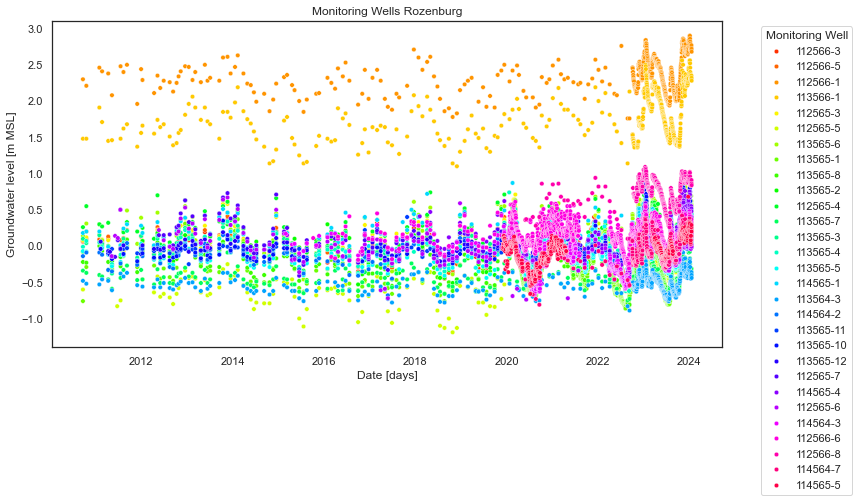
\includegraphics[width=0.80\linewidth]{frontmatter/Rozenburg-fig/rozscatter.png}
    \caption{Observed data for 29 monitoring wells in Rozenburg.}
    \label{beforeroz}
\end{figure}\\

\subsection{Pastas Time Series Modeling}
The bar plot displays the recharge rates in m/day over a period from 2010 to 2024. The x-axis represents the time period from 2010-2024 with the dates labeled on the x-axis. The y-axis quantifies the recharge rate, with values ranging from 0 to a maximum of 0.07 m/day. The bars shows the variability in recharge rates over time, where some years experience peaks in recharge (higher recharge rates), which can be due to increased precipitation. As can be seen from \labelcref{recharge}, the data is dense, indicating frequent measurements. The pattern of the bars reflects seasonal changes. Lower values are more frequently observed, possibly indicating a baseline level of recharge over the years. Two additional figures (\labelcref{P} and \labelcref{ET}) of the precipitation and potential evaporation are visualized as well. The data of these figures is combined to determine the recharge rate in the municipal area.


\begin{figure}[htbp]
    \centering
    \includegraphics[width=0.80\linewidth]{frontmatter/Rozenburg-fig/Recharge.png}
    \caption{Recharge [m/day] over a period of 2010-2024, measured by KNMI weather station 344 in Rotterdam, The Netherlands.}
    \label{recharge}
\end{figure}

\begin{figure}[htbp]
    \centering
    % First figure
    \begin{minipage}{0.45\textwidth}
        \centering
        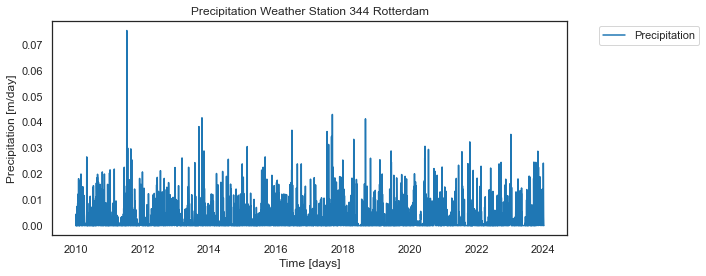
\includegraphics[width=\linewidth]{frontmatter/Heijplaat-fig/P.png}
        \caption{Precipitation [m/day] over a period of 2010-2024, measured by KNMI weather station 344 in Rotterdam, The Netherlands. }
        \label{P}
    \end{minipage}\hfill
    % Second figure
    \begin{minipage}{0.45\textwidth}
        \centering
        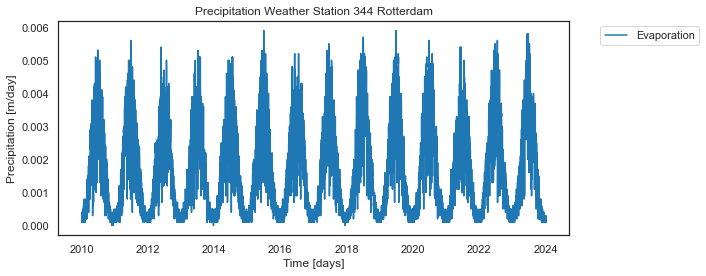
\includegraphics[width=\linewidth]{frontmatter/Heijplaat-fig/ET.png}
        \caption{Potential evaporation [m/day] over a period of 2010-2024, measured by KNMI weather station 344 in Rotterdam, The Netherlands.}
        \label{ET}
    \end{minipage}
\end{figure}

\subsubsection{Reverse forecasting}
A part of the Pastas package is reverse forecasting or also called backcasting of the observed data. Reversed forecasting takes place for all the unique monitoring wells present in the case study area. For every monitoring well, three figures are created: a) Reversed backcasting for data loggers; b) Reversed backcasting for manual measurements; c) A combination figure of the two figures combined, see figures \labelcref{dl}-\labelcref{combi}. An example is shown for monitoring well 114564-7.

\begin{figure}[htbp]
    \centering
    % First figure
    \begin{minipage}{0.32\textwidth}
        \centering
        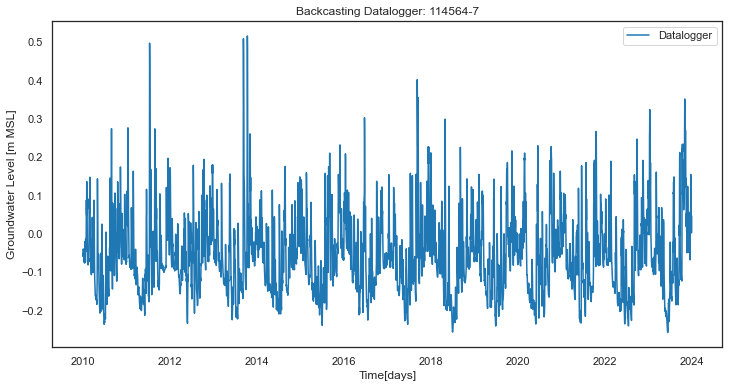
\includegraphics[width=\linewidth]{frontmatter/Rozenburg-fig/pastasdl.png}
        \caption{Reversed forecasting data based on datalogger data for monitoring well 114564-7.}
        \label{dl}
    \end{minipage}
    \hfill
    % Second figure
    \begin{minipage}{0.32\textwidth}
        \centering
        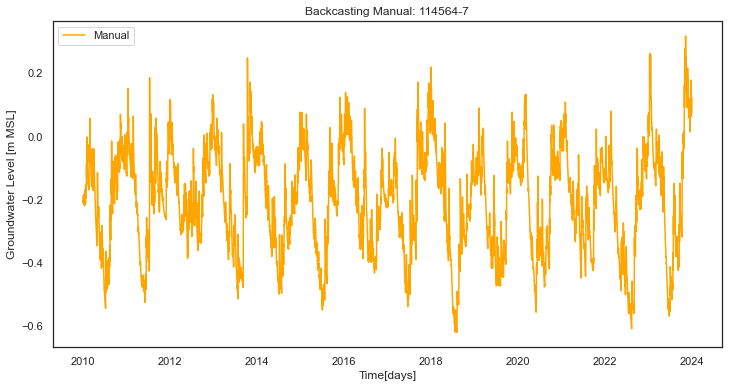
\includegraphics[width=\linewidth]{frontmatter/Rozenburg-fig/pastasman.png}
        \caption{Reversed forecasting data based on manual measurement data for monitoring well 114564-7.}
        \label{hp}
    \end{minipage}
    \hfill
    % Third figure
    \begin{minipage}{0.32\textwidth}
        \centering
        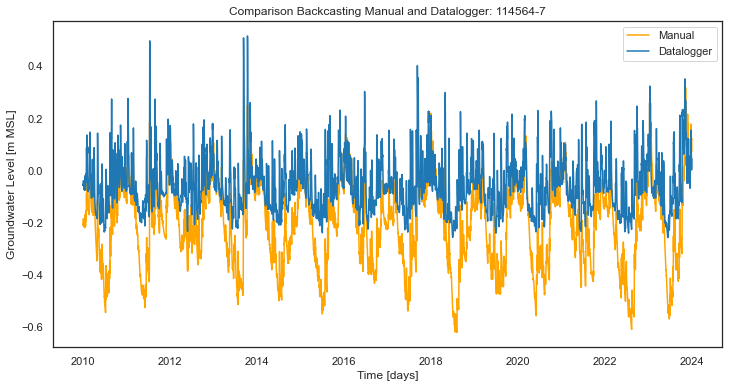
\includegraphics[width=\linewidth]{frontmatter/Rozenburg-fig/pastascombi.png}
        \caption{Reversed forecasting data based on manual measurement data and datalogger data for monitoring well 114564-7.}
        \label{combi}
    \end{minipage}
\end{figure} \\

\subsubsection{Performance metrics}
The bar plot (\labelcref{bar1} and \labelcref{bar2} shows the two metrics RMSE and R2 for all unique monitoring wells. 4 Categories are shown: manual-rmse, manual-rsq, datalogger-rmse, datalogger-rsq. The RMSE seems to be high for some monitoring wells, which could be explained by a high reconstruction error in both of the measurement types. Generally, it looks like the R2 values of the manual measurements are higher than the values of the data loggers. This could suggest that the manual measurements could provide a better fit with the simulated results. The fit of the RMSE and R2 differ for every monitoring well, meaning that there is not a specific pattern that suggests if one of the data groups performs better. An additional bar plot, fig. \labelcref{barevp}, describes the EVP [\%] cross the data set. The EVP is a goodness-of-fit indicator which compares the variance of the observed data and the variance of the residual data (Asmuth von et al., 2012). A low EVP indicates that data could be missing in the data set, where the spatial pattern could be a possible reason. A statistical t-test is a follow up, because this can test scientifically and statistically substantiate the difference in performance between the two data groups.  
\newline
Based on the results of the bar plot, the decision was made to execute further statistical tests. A Welch's t-test was carried out, leading to the following results. The Welch's t-test uses an alpha equal to 0.05. 

\begin{figure}[h]
    \centering
    \begin{minipage}{0.48\textwidth}
        \centering
        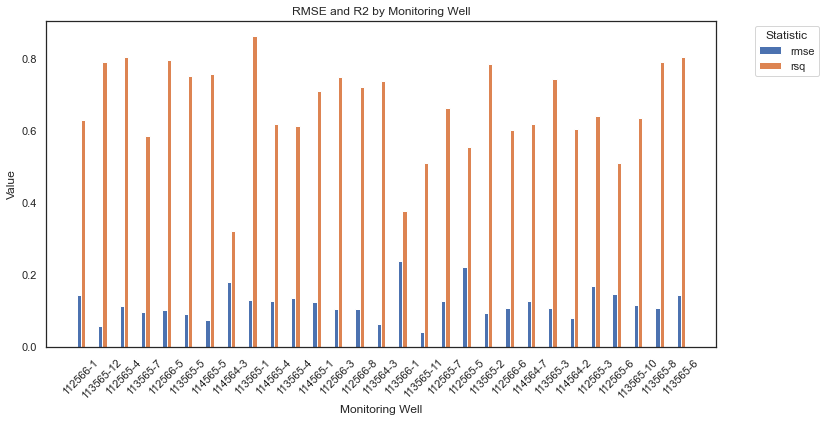
\includegraphics[width=\linewidth]{frontmatter/Rozenburg-fig/rmser2roz.png} % Adjust the file name or path as needed.
        \caption{Bar plot showing the metrics RMSE and $R^2$ for 29 monitoring wells.}
        \label{bar1}
    \end{minipage}\hfill
    \begin{minipage}{0.48\textwidth}
        \centering
        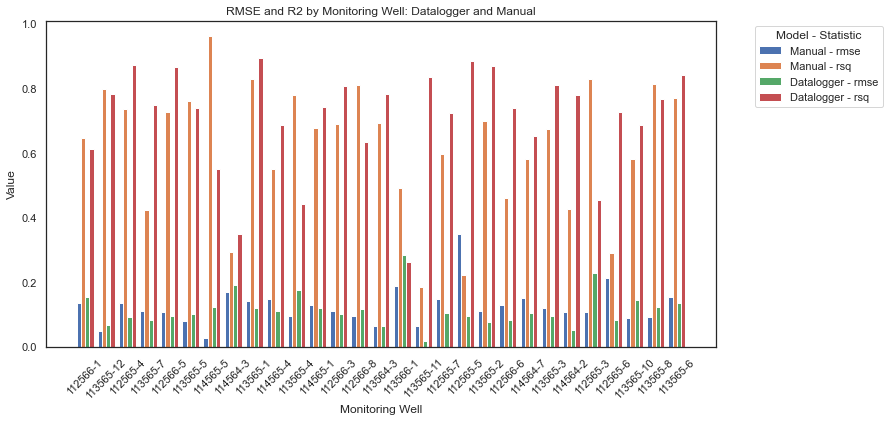
\includegraphics[width=\linewidth]{frontmatter/Rozenburg-fig/rmser2roz2.png} % Adjust the file name or path as needed.
        \caption{Bar plot showing metrics RMSE and $R^2$ for 29 monitoring wells with a division in data logger and manual collection method.}
        \label{bar2}
    \end{minipage}
\end{figure}

\begin{figure}[h]
    \centering
    \begin{minipage}{0.48\textwidth}
        \centering
        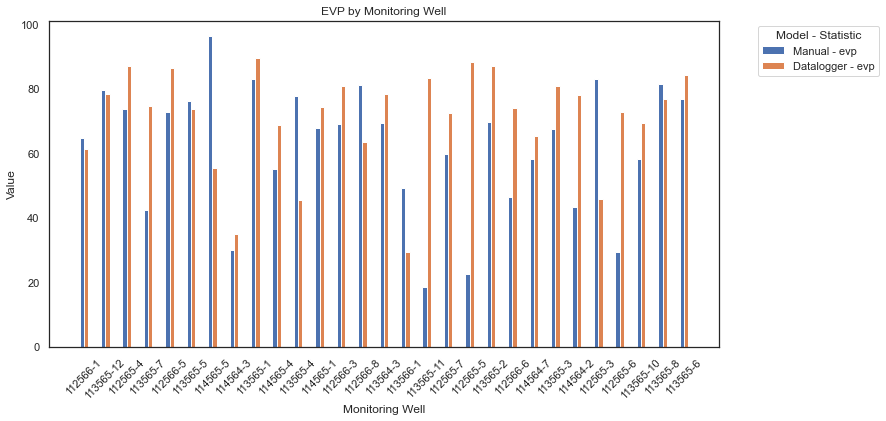
\includegraphics[width=\linewidth]{frontmatter/Rozenburg-fig/evproz2.png} % Adjust the file name or path as needed.
        \caption{Bar plot showing metric EVP for 29 monitoring wells.}
        \label{barevp}
    \end{minipage}\hfill
\end{figure}
Figure \labelcref{welch} displays the result of the Welch's t-test, based on alpha = 0.5. The results of the performance metrics are labeled as RMSE, R2, and EVP. Each performance metric provides the results of the t-statistic and p-value of the Welch's statistical test. The RMSE (blue section), explains that the t-statistic is negative. This result could indicate that the dataloggers has a lower mean RMSE than the manual collection method. The p-value is higher than alpha = 0.05. A p-value higher than the set alpha explains that no significant difference is present between the dataloggers and manual collection method. The R2 (orange section) explains that the t-statistic is positive, indicating a higher mean R2 for the dataloggers than the manual collection method. The p-value is slightly higher than alpha = 0.05, indicating no significant difference. The last metric is the EVP (green section). The t-statistic of the EVP has a positive value, suggesting that the dataloggers might have a higher mean EVP than the manual collection method. The p-value of 0.065 is very close to 0.05, but resulting in no significant difference. 

\begin{figure}[htbp]
    \centering
    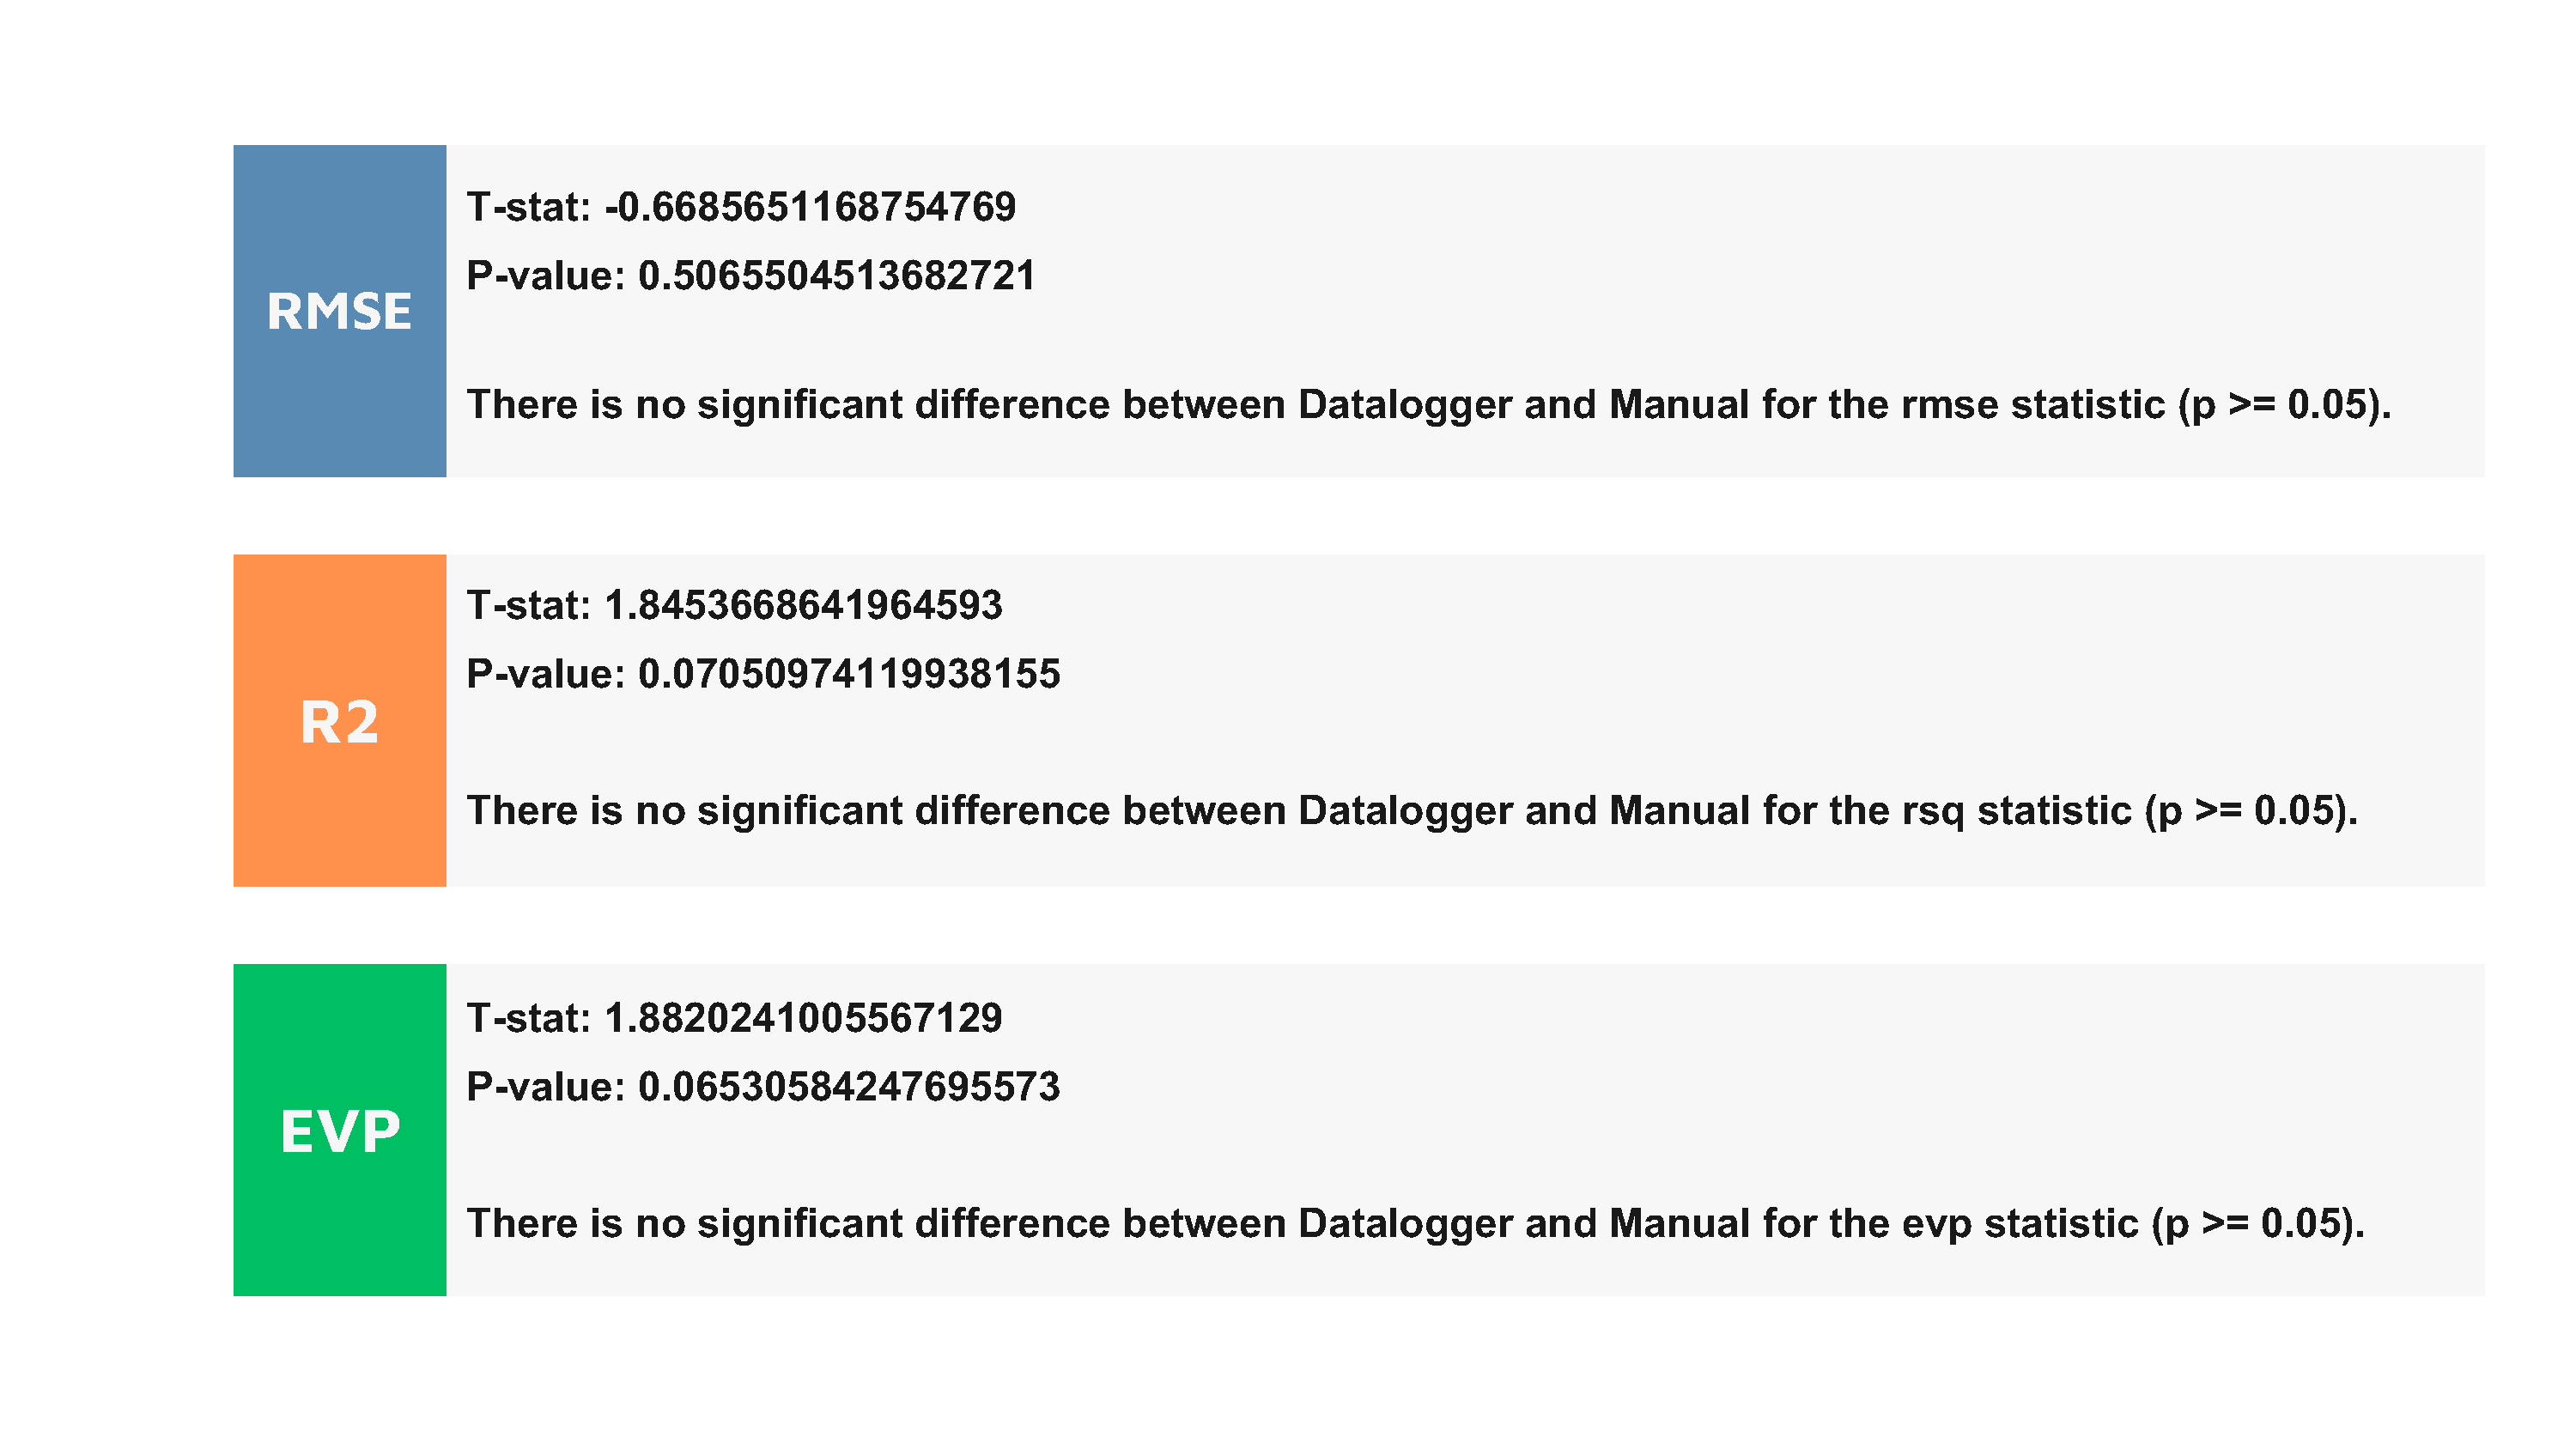
\includegraphics[width=0.80\linewidth]{frontmatter/Rozenburg-fig/rozstat.pdf}
    \caption{Overview of the performance of RMSE, $R^2$ , and EVP after the Welch's t-test and the difference between data loggers and manual collection method. }
    \label{welch}
\end{figure}
\newpage
According to the Welch's t-test, no substantial discrepancies were found in the data groups. None of the P-values are below the cut-off of alpha = 0.05. Consequently, it was decided to proceed with the group that is specialized in data loggers. Despite statistical significance, other factors are crucial in environmental sciences. Hence, the datalogger group is chosen, merging observed and simulated data into one dataset and excluding the manual measurements. 

\subsubsection{Creation of new data frame}
Scatter plot \labelcref{scatter} below, visualizes the observed data logger with the pink scatter and the simulated data of the data logger is visualized by the green scatter. On the x-axis the time period [days] is shown and on the y-axis the groundwater level [m MSL]. Figure \labelcref{scatter} visualizes only monitoring well 114564-7, the remaining monitoring wells of the neighborhood Rozenburg are available in the appendix and through GitHub.

\begin{figure}[htbp]
    \centering
    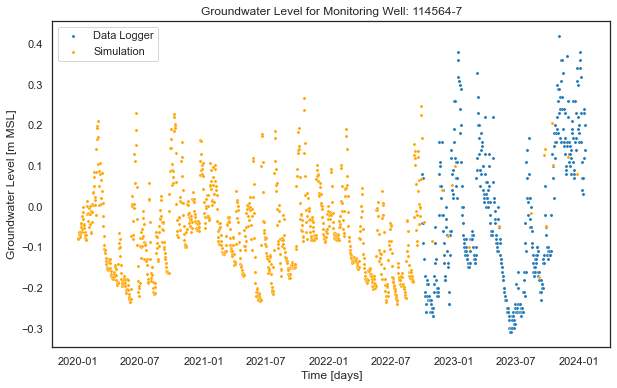
\includegraphics[width=0.80\linewidth]{frontmatter/Rozenburg-fig/scatterpastasex.png}
    \caption{Scatter plot of simulated and observed data by data loggers for monitoring well 114564-7. The x-axis shows a period of 2020-2024 and the y-axis shows a range of -0.3 to 0.4 meters MSL. }
    \label{scatter}
\end{figure}

\clearpage

\subsection{QR factorization}
Using QR factorization as a foundation, a hierarchical list of the monitoring wells in Rozenburg is created. The optimal reduction percentage is determined and reduction tests can be executed. Resulting in an overview of eliminated monitoring wells and their capability to reconstruct future groundwater levels in the network.

\subsubsection{1D hydrograph data}
Figure \labelcref{gwlroz} is a geographical representation (epsg=28992) visualizing the spatial distribution of monitoring wells in the neighborhood "Rozenburg". Within the map, a scatter plot with a color scale represents the groundwater level measurements taken at the monitoring wells. The color scale has a range between -0.5 m to +2.0 m MSL. Each monitoring well represents a location as well as the color of monitoring well represents the value on the color scale. At the north side of the neighborhood, deviating groundwater level measurements can occur because of the elevation difference of the ground level, a digital terrain model of Rozenburg is displayed in figure \labelcref{AHNroz}.
\begin{figure}[htbp]
    \centering
    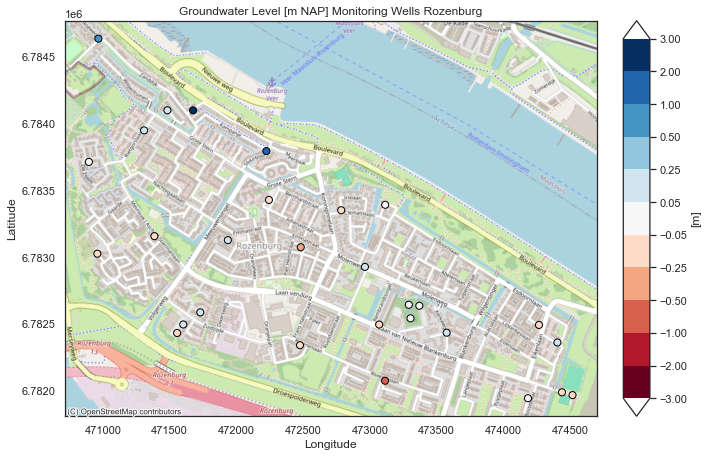
\includegraphics[width=0.80\linewidth]{frontmatter/Rozenburg-fig/gwlroz.png}
    \caption{Groundwater level [m MSL] across Rozenburg, using a color-coded system to represent the mean GWL observations for the 29 monitoring wells. }
    \label{gwlroz}
    
\end{figure}

\subsubsection{Sampling data}
Preprocessing of the data includes transforming the data frame into an array, implementing both global and local centering methods, and splitting the dataset into an 80/20 ratio training and test set distribution. The result of the preprocessing is as follows, see table \labelcref{data}
\begin{table}[htbp]
\centering
\caption{Summary of sampling data.}
\label{data}
\begin{tabular}{|l|l|}
\hline
\textbf{Parameter}                           & \textbf{Value}                                \\ \hline
Sampling period                              & 2010-09-02 00:00:00 to 2023-12-31 00:00:00   \\ \hline
Number of samples                            & 4870                                          \\ \hline
Number of features (sensors)                 & 29                                            \\ \hline
Shape of X (samples, sensors)                & (4870, 29)                                    \\ \hline
Min. and max. value                          & -0.8734088406515021 [m] ; 2.857148050691837 [m] \\ \hline
Min. and max. centered value                 & -0.544 [m] 0.732 [m]                         \\ \hline
Min. and max. centered value (exact)         & -0.5436141745216054 [m], 0.7315291423503969 [m] \\ \hline
Mean centered data                           & -0.0 [m]                                     \\ \hline
Train data, Test data                        & 3896 , 974                                   \\ \hline
Train data, Test data (percentage)           & 80\%, 20\%                                  \\ \hline
\end{tabular}
\end{table} 

\subsubsection{Hierarchy of monitoring wells}
A geographical representation (epsg=28992) of data points plotted on a x,y coordinate system is visualized in figure \labelcref{rankroz}. The horizontal axis is labeled as longitude and the vertical axis is labeled as latitude. The data points are scattered across the study area within a polygonal boundary that represents the neighborhood "Rozenburg". Each monitoring well monitoring well is color-coded according to the color bar on the right side of the plot. The color indicates the rank of each monitoring well. The color bar has a range between dark blue for the lowest values (0) to yellow for the highest values (29). The distribution of the color code does not follow a clear pattern within the polygonal boundary. Some clusters of higher or lower ranked monitoring wells are present. Overall, the monitoring wells with additional value are marked blue. They show possibly show flashiness in their data, meaning a high frequency and rapidity in short term changes with strong irregular patterns. According to Ohmer et al. (2022), these monitoring wells indicate strong interaction with surface waters and boundary inflows. As well as a high seasonality and low variability. The monitoring wells that likely do not have additional value to the network are marked yellow. These wells show low flashiness and high seasonality. The most redundant monitoring wells appear to be located towards the southern edge of the polygonal boundary. At this site, the monitoring wells are clustered, addressing a region of low data variability and flashiness. As well as one single monitoring well in the north of the area. For this monitoring well it does not seem clear why this monitoring wells is redundant, based on other factors as seasonality and flashiness. 

\begin{figure}[h]
    \centering
    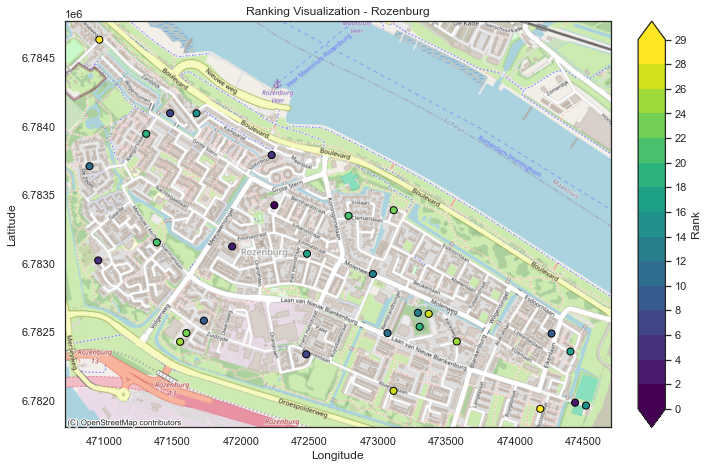
\includegraphics[width=0.8\linewidth]{frontmatter/Rozenburg-fig/rankroz.png}
    \caption{Visualization of the hierarchical list of 29 monitoring wells across Rozenburg.}
    \label{rankroz}
\end{figure} 

\newpage

\subsubsection{Determining the optimal reduction rate}
In figures \labelcref{roz10} - \labelcref{roz90} , the reconstruction error of Rozenburg is displayed, plotting the root mean square error (RMSE) in meters on the y-axis against the number of monitoring wells on the x-axis. The line graph shows a decreasing function in the RMSE as the number of monitoring wells increases, suggesting that more monitoring wells contribute to a lower reconstruction error in the data. In the figures, the orange marked point marks the optimal number of monitoring wells where the reconstruction error reaches the threshold that is indicated by the orange line. The threshold is an acceptable level of RMSE for the reconstruction process. The original groundwater monitoring network of Rozenburg includes 29 monitoring wells.
\newline
Starting with figure \labelcref{roz10}, a reduction of 10\% describes that 26 monitoring wells remain in the network and only 3 monitoring wells might be eliminated. The reconstruction error reaches a value below 0.02 meters. The RMSE in figure \labelcref{roz25}, a reduction of 25\% explains that a number of 21 monitoring wells is the most optimal with a removal of 8 monitoring wells.  Figure \labelcref{roz50}, demonstrates a function, based on a reduction rate of 50\%. The RMSE decreases as more monitoring wells are added to the network. At the point of n=14 on the x-axis, an orange dot is indicated. Beyond this point, the decrease in RMSE slows down, suggesting returns on error reduction after a specific number of monitoring wells is reached. 

\begin{figure}[htbp]
    \centering
    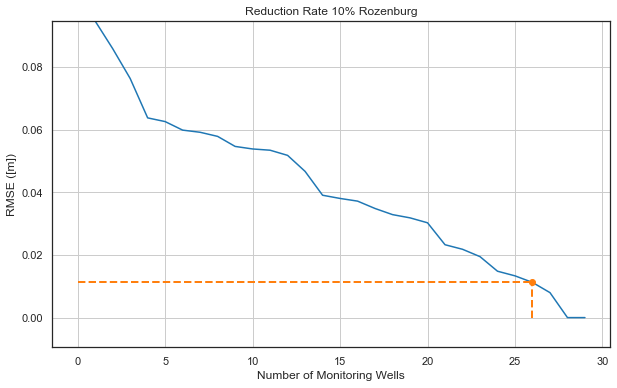
\includegraphics[width=0.48\linewidth]{frontmatter/Rozenburg-fig/rozenburg10.png}
    \caption{RMSE based on a network reduction of 10\%. The optimal number of wells is 26.}
    \label{roz10}
\end{figure}

    % Second Figure
    \begin{figure}[htbp]
    \begin{minipage}{0.48\textwidth}
        \centering % Centers the content of this minipage
        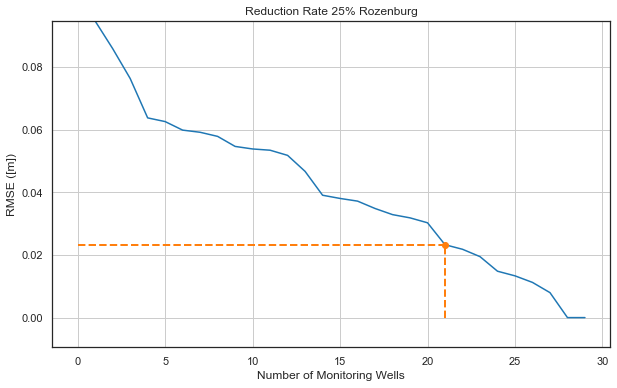
\includegraphics[width=\linewidth]{figures/res roz/25roz.png}
        \caption{RMSE based on a network reduction of 25\%. The optimal number of wells is 21.}
        \label{roz25}
    \end{minipage}
    % Third Figure
    \begin{minipage}{0.48\textwidth}
        \centering % Centers the content of this minipage
        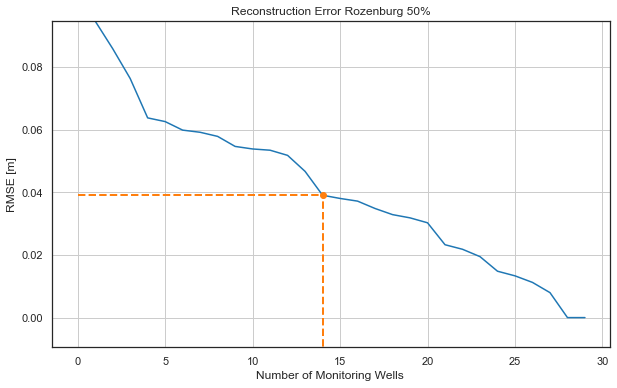
\includegraphics[width=\linewidth]{figures/res roz/50roz.png}
        \caption{RMSE based on a network reduction of 50\%. The optimal number of wells is 14.}
        \label{roz50}
    \end{minipage}
\end{figure}

\newpage
Figure \labelcref{roz75} displays a function where the RMSE decreases as the number of monitoring wells increases. The RMSE sharply declines as the monitoring well count approach reaches the point above 10 monitoring wells. This point is marked by the orange dashed line. The line marks the optimal number of monitoring wells where the reconstruction error reaches the threshold value. The threshold value is determined by the trade off between the maximum information value and minimum cost, in which the maximum information is characterized by the reconstruction error and the minimum cost is equivalent to the number of monitoring wells. Initially, Rozenburg includes 29 monitoring wells. The results of the RMSE explain that only 7 monitoring wells will remain, 22 monitoring wells have to be removed from the local network if a reduction of 75\% is used in the approach. A reduction rate of 75\% explains an equilibrium state between the number of monitoring wells and the reconstruction error that is achieved.
\newline
Continuing with figure \labelcref{roz90}, the reconstruction error for a reduction of 90\% is displayed. The figure plots the RMSE in meters on the y-axis against the number of monitoring wells on the x-axis. The line graph shows a sharp decreasing function in the RMSE as the number of monitoring wells increases. The orange marked point marks the optimal number of monitoring wells where the reconstruction error reaches the threshold that is indicated by the orange line. The threshold is an acceptable level of RMSE for the reconstruction process. Initially, Rozenburg has 29 monitoring wells. The results of the RMSE calculation explains that a number of 2 monitoring wells will remain with this reduction rate, 27 monitoring wells will be removed from the local network. 


\begin{figure}[htbp]
    \centering
    \begin{minipage}{0.48\textwidth}
        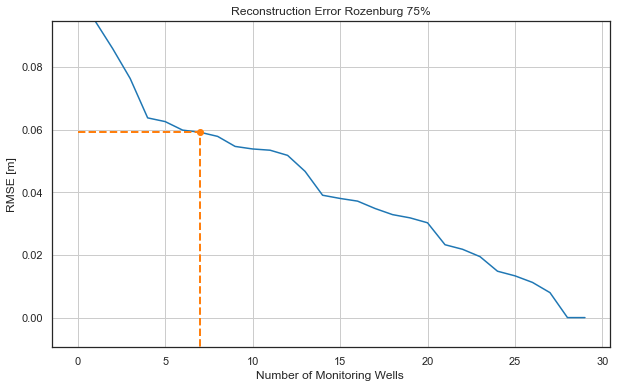
\includegraphics[width=\linewidth]{figures/res roz/75roz.png}
        \caption{RMSE based on a network reduction of 75\%. The optimal number of wells is 7.}
        \label{roz75}
    \end{minipage}\hfill
    \begin{minipage}{0.48\textwidth}
        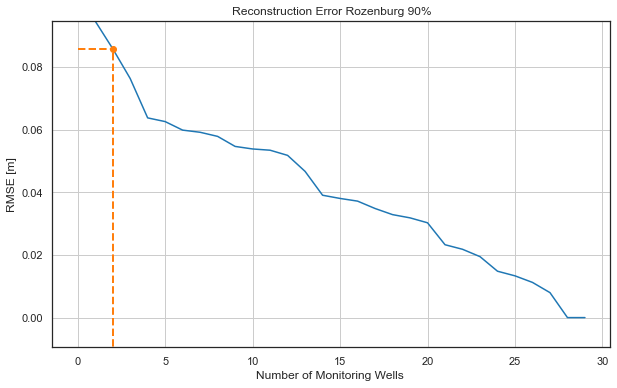
\includegraphics[width=\linewidth]{figures/res roz/90roz.png}
        \caption{RMSE based on a network reduction of 90\%. The optimal number of wells is 2.}
        \label{roz90}
    \end{minipage}
\end{figure}


\subsubsection{The optimal reduction rate}
The optimal reduction rate for a monitoring network consisting of 29 monitoring wells counts up to a value where both RMSE and MAE reach a stabilization. Figure \labelcref{rmse} visualizes all reduction rates between a range of 10-90\% with their corresponding reconstruction error and mean absolute error. The upper values of each reduction rate correlate to the MAE, while the lower values, with the connecting dashed-line describes the reconstruction error. \\
\\
A reduction rate of 25\% implies that the optimal number of monitoring wells is 21, meaning that 8 monitoring wells might be eliminated, see figure \labelcref{roz25}. Additionally, the RMSE counts up to 0.1 and the MAE to 0.18 meters. 
\begin{figure}[htbp]
    \centering
    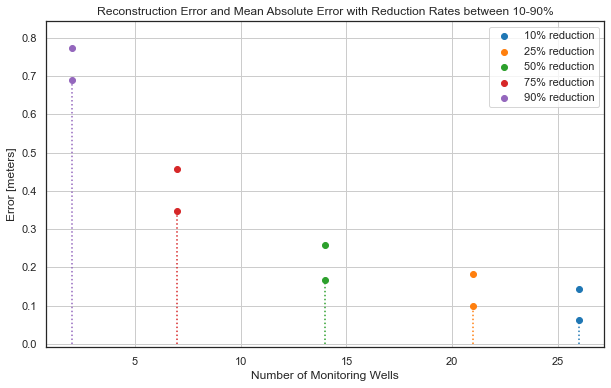
\includegraphics[width=0.5\linewidth]{frontmatter/Rozenburg-fig/errorroz.png}
    \caption{Overview of the RMSE and MAE for a range of reduction rates (10-25-50-75-90 \%). }
    \label{rmse}
\end{figure}
As stated in the chapter \textit{Research Methodology}, the reconstruction capability of the eliminated monitoring wells is tested through the creation of hydrographs. In figures \labelcref{roz1}-\labelcref{roz8}, hydrographs are shown. The hydrographs include a measured (blue line) and reconstructed (red line) function. The reconstructed functions are based on observed data and the goodness-of-fit of the model. Performance metrics regarding the MAE, RMSE, R2, and rBIAS determine the goodness-of-fit of the functions, they are available underneath the figures \labelcref{roz1}-\labelcref{roz8}. 
\newpage
As can be seen from the figures, the plots have a comparable function; a decreasing groundwater level from April 2023 on and reaching the lowest groundwater level in July 2023. In August 2023, the groundwater level increases again to high levels. At the end of August 2023, the groundwater level decreases again, but experiences peak values in October 2023. At the end of 2023, the groundwater levels are increasing again, but at this time of the year, the levels look more constant. Based on the performance metrics of the potentially eliminated monitoring wells, it can be seen that the MAE and RMSE are constant values throughout the network. The MAE reaches a value of 0.04 meters and the RMSE counts up to 0.05 meters. The coefficient of determination differs for every monitoring well, but ranges between 0.87 and 0.99 meters. An average R2 of 0.95 meters is calculated.

\begin{figure}[h]
    \centering
    % Row 1
    \begin{minipage}{0.48\textwidth}
        \centering
        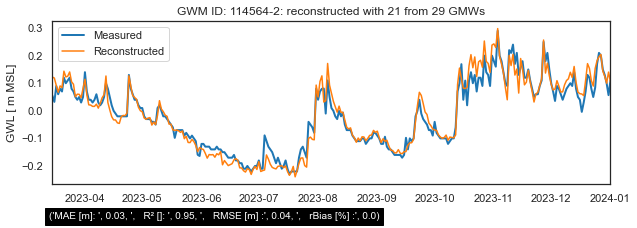
\includegraphics[width=\linewidth]{frontmatter/Rozenburg-fig/1145642.png}
        \caption{Eliminated monitoring well: 114564-2.}
        \label{roz1}
    \end{minipage}\hfill
    \begin{minipage}{0.48\textwidth}
        \centering
        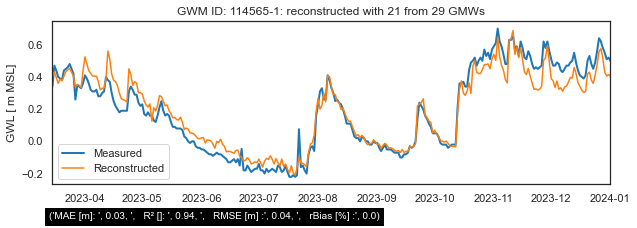
\includegraphics[width=\linewidth]{frontmatter/Rozenburg-fig/1145651.png}
        \caption{Eliminated monitoring well: 114565-1. }
        \label{114565-1}
    \end{minipage}
    
    % Row 2
    \begin{minipage}{0.48\textwidth}
        \centering
        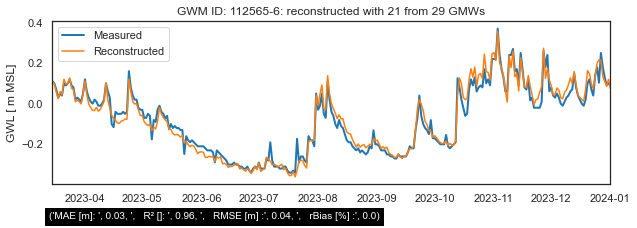
\includegraphics[width=\linewidth]{frontmatter/Rozenburg-fig/1125656.png}
        \caption{Eliminated monitoring well: 112565-6.}
        \label{112565-6}
    \end{minipage}\hfill
    \begin{minipage}{0.48\textwidth}
        \centering
        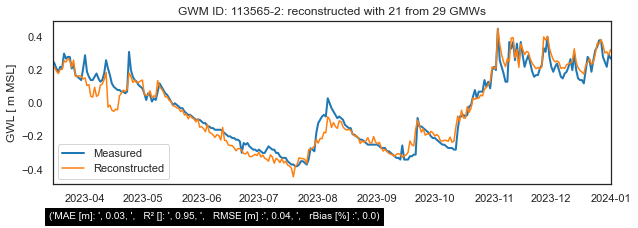
\includegraphics[width=\linewidth]{frontmatter/Rozenburg-fig/1135652.png}
        \caption{Eliminated monitoring well: 113565-2.}
        \label{113565-2}
    \end{minipage}
    % Row 3
    \begin{minipage}{0.48\textwidth}
        \centering
        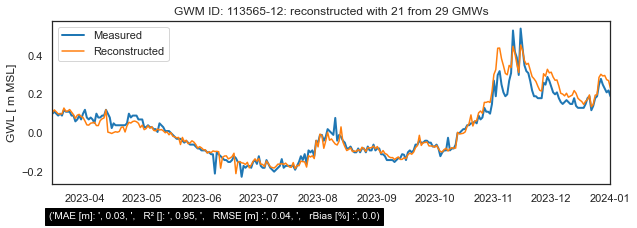
\includegraphics[width=\linewidth]{frontmatter/Rozenburg-fig/11356512.png}
        \caption{Eliminated monitoring well: 113565-12.}
        \label{113565-12}
    \end{minipage}\hfill
    \begin{minipage}{0.48\textwidth}
        \centering
        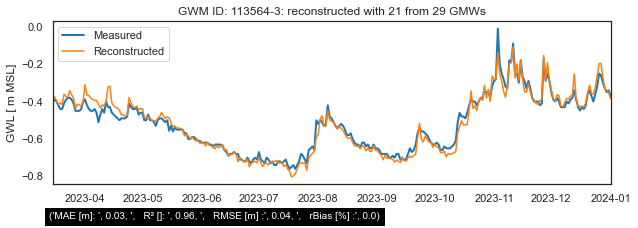
\includegraphics[width=\linewidth]{frontmatter/Rozenburg-fig/1135643.png}
        \caption{Eliminated monitoring well: 113564-3.}
        \label{113564-3}
    \end{minipage}

    % Row 4
    \begin{minipage}{0.48\textwidth}
        \centering
        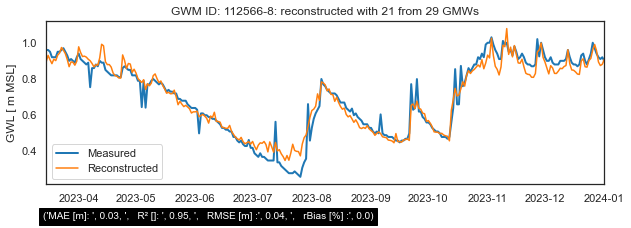
\includegraphics[width=\linewidth]{frontmatter/Rozenburg-fig/1125668.png}
        \caption{Eliminated monitoring well: 112566-8.}
        \label{112566-8}
    \end{minipage}\hfill
    \begin{minipage}{0.48\textwidth}
        \centering
        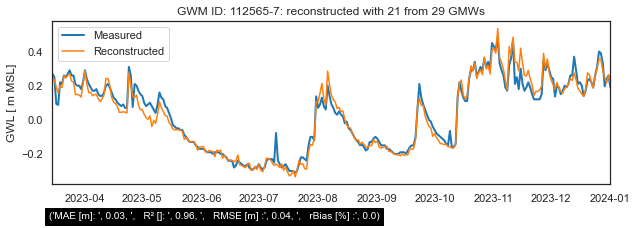
\includegraphics[width=\linewidth]{frontmatter/Rozenburg-fig/1125657.png}
        \caption{Eliminated monitoring well: 112565-7.}
        \label{roz8}
    \end{minipage}
\end{figure}\\
\\
The measured and reconstructed groundwater levels are tested with the Welch's t-test to determine whether it is the case of a significant difference between the measured and reconstructed groundwater levels. The results are displayed in table \labelcref{welchroz}. Only 4 out of the 10 eliminated monitoring wells experiences a significant difference between the measured and reconstructed groundwater level data. This means that the p-values of the monitoring wells are lower than alpha = 0.05. 
\begin{table}
    \centering
      \caption{Overview of statistical results of the eliminated monitoring wells with a network reduction of 25\%. The overview explains the p-value of the monitoring wells and if they experience a significant difference between the observed and reconstructed data.}
    \begin{tabular}{|c|c|} \hline 
         Monitoring Well& Result t-Test\\ \hline 
         112565-6& No significant difference (p-value = 0.328)\\ \hline 
         112565-7& Significant difference (p-value = 0.008)\\ \hline 
         112566-8& No significant difference (p-value = 0.879)\\ \hline 
         113564-3& No significant difference (p-value = 0.551)\\ \hline 
         113565-12& Significant difference (p-value = 0.001)\\ \hline 
         113565-2& Significant difference (p-value = 0.008)\\ \hline 
         114564-2& No significant difference (p-value = 0.155)\\ \hline 
         114565-1& No significant difference (p-value = 0.342)\\ \hline
    \end{tabular}

    \label{welchroz}
\end{table}

\clearpage
Figure \labelcref{rozbox} visualizes a box plot that displays the distribution of the performance metric R2, the coefficient of determination, across the dataset, after reduction of 25\% took place. On the y-axis, the score in meters is shown, which ranges between 0.939 and 0.9645. The red line explains a median value of around 0.951 meters. The whiskers at the bottom and top of the box do not have equal length. The whisker the bottom reaches a value up to 0.939 meters to a score of 0.9645 meters. The box itself ranges between 0.948 and 0.962 meters. 

\begin{figure}[htbp]
    \centering
    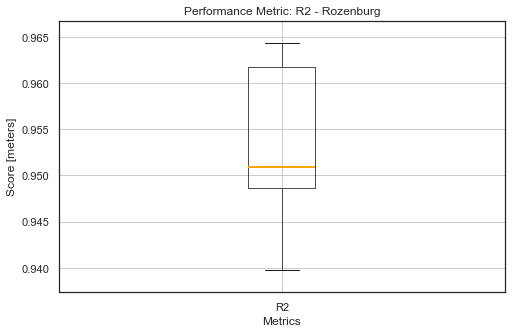
\includegraphics[width=0.5\linewidth]{frontmatter/Rozenburg-fig/R2box.png}
    \caption{Performance metric $R^2$ for Rozenburg. 
    The orange line indicates the median value. The y-axis ranges from X to X meters.}
    \label{rozbox}
\end{figure}

\subsubsection{Mean Absolute Error of Reduction}
Based on a reduction percentage of 25\%, reconstruction hydrographs could be plotted in figures \labelcref{roz1}-\labelcref{roz8}. The extent to which the reconstructed groundwater level data corresponds to the actual observed data can be determined by the mean absolute error [meters]. The mean absolute error is calculated for every, eliminated monitoring well. A color rank is visualized in figure \labelcref{maeroz} with the level of the calculated mean absolute error (epsg=28992). Blue indicates a low MAE, while yellow indicates a high MAE. The visualization enables the identification of monitoring wells with higher or lower predictive accuracy, which could influence decision-making regarding the placement of future monitoring wells or the scope of maintenance efforts on existing wells. The MAE measures indirectly the performance of the monitoring well regarding data reconstruction. A high MAE in a network of lower MAE values can suggest a vulnerable monitoring well for external, environmental factors. Monitoring wells with a high MAE address the reliability of the data. The monitoring well that is marked with a yellow color indicates a higher MAE value compared to the other monitoring wells. 

\begin{figure}[htbp]
    \centering
    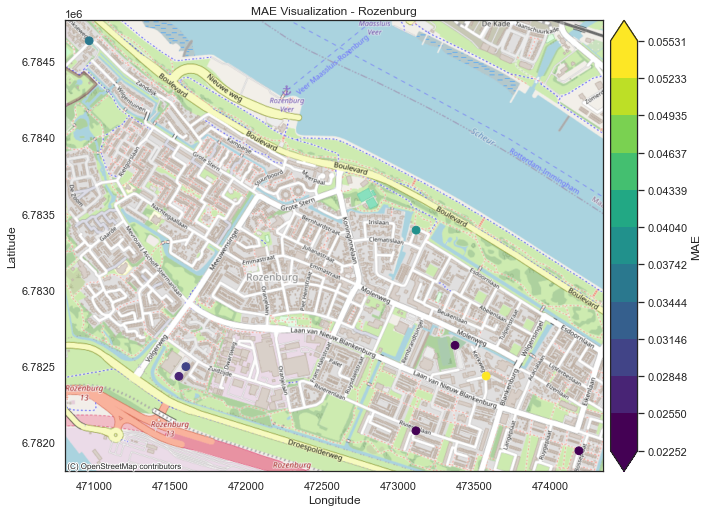
\includegraphics[width=1\linewidth]{frontmatter/Rozenburg-fig/mae25roz.png}
    \caption{Mean Absolute Error [meters] across Rozenburg, using a color-coded system to represent the calculated MAE for the eliminated monitoring wells.}
    \label{maeroz}
\end{figure}

\clearpage

\subsubsection{Remaining Network}
After the network is reduced, 75\% of the monitoring wells will remain in the GWMN after reduction takes place. A geographical representation (epsg=28992) of the monitoring wells is available in figure \labelcref{afterroz} The blue sites indicate the location of the existing monitoring wells. Initially, the GWMN of Rozenburg had a density of one monitoring well/54.34 $m^2$. After the reduction-optimization process, the network changes to one monitoring well/75.647 $m^2$. 

\begin{figure}[htbp]
    \centering
    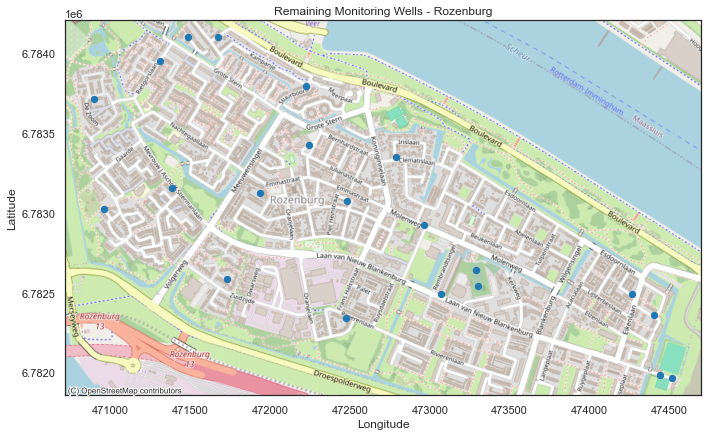
\includegraphics[width=1\linewidth]{frontmatter/Rozenburg-fig/After.png}
    \caption{Map depiction of the remaining monitoring wells in Rozenburg after following a 25\% reduction of the network. }
    \label{afterroz}
    
\end{figure}

\clearpage

\section{Heijplaat}
\subsection{QGIS and PROWAT}

A multi-colored scatter plot is represented, showing the groundwater level [m MSL] over time [days] for the neighborhood "Heijplaat" in figure \labelcref{summheij}. The x-axis is broad, ranging from 1980 to 2024. Heijplaat has much historical groundwater data available. Each colored dot represents an individual data point from a unique monitoring well, see legend on the right side of the figure. A wide array of groundwater levels is depicted, ranging from below +1.0 to little points of +3.5 m MSL. 
\\
\\
Plot \labelcref{summheij} visualizes variation in groundwater levels between different monitoring wells. Some of the monitoring wells perform more stable groundwater levels, while other monitoring wells have an abundant fluctuation. Dense clustering of data points suggests that measurements were taken frequently over that period of time. The variety of colors that are connected to the individual monitoring wells allows the possibility for a comparison of groundwater level functions between monitoring locations within the neighborhood. \\
\begin{figure}[htbp]
    \centering
    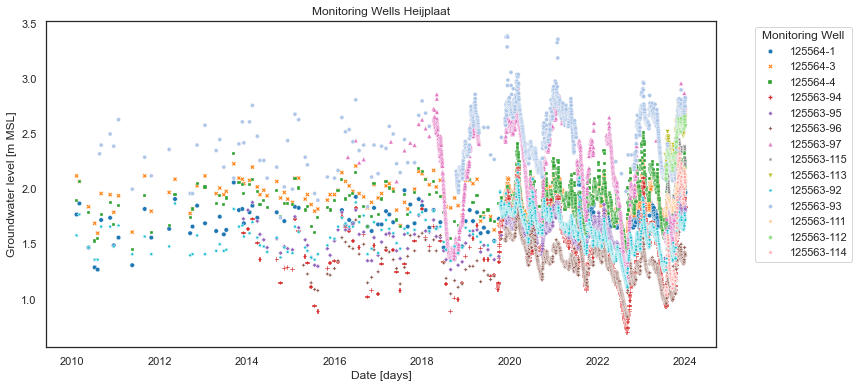
\includegraphics[width=0.75\linewidth]{frontmatter/Heijplaat-fig/heijoverzicht.png}
    \caption{Observed data for 14 monitoring wells in Heijplaat.}
    \label{summheij}
\end{figure}\\

\subsection{Pastas time series modeling}
Similarly to the plot in the section "Rozenburg", the bar plot displays the recharge rates in m/day over a period from 2010 to 2024, figure \labelcref{R} The y-axis quantifies the recharge rate, with values ranging from 0 to 0.07 m/day. The bars show variability in recharge rates over time, where some years experience peaks in recharge (higher recharge rates), which can be due to increased precipitation. As can be seen from the figure, the data is dense, indicating frequent measurements. The pattern of the bars reflect seasonal changes. Lower values of recharge are more frequently observed than high outliers, possibly indicating a baseline level of recharge over the years. Two additional figures of the precipitation (\labelcref{P}) and potential evaporation (\labelcref{ET}) are visualized as well. The data of these figures is combined to determine the recharge rate in the municipal area. 

\begin{figure}[htbp]
    \centering
    \includegraphics[width=0.75\linewidth]{frontmatter/Heijplaat-fig/Recharge.png}
    \caption{Recharge [m/day] over a period of 2010-2024, measured by KNMI weather station 344 in Rotterdam, The Netherlands.}
    \label{R}
\end{figure} 
\vspace{0.5cm}
\begin{figure}[h]
    \centering
    % First figure
    \begin{minipage}{0.45\textwidth}
        \centering
        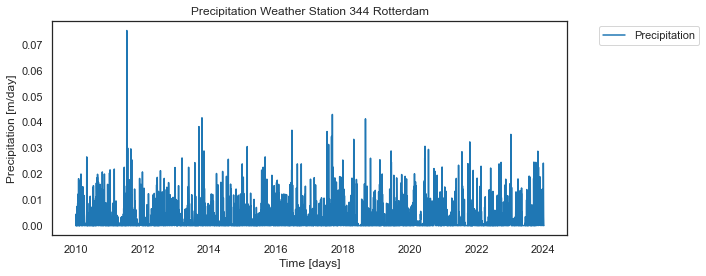
\includegraphics[width=\linewidth]{frontmatter/Heijplaat-fig/P.png}
        \caption{Precipitation [m/day] over a period of 2010-2024, measured by KNMI weather station 344 in Rotterdam, The Netherlands.}
        \label{P}
    \end{minipage}\hfill
    % Second figure
    \begin{minipage}{0.45\textwidth}
        \centering
        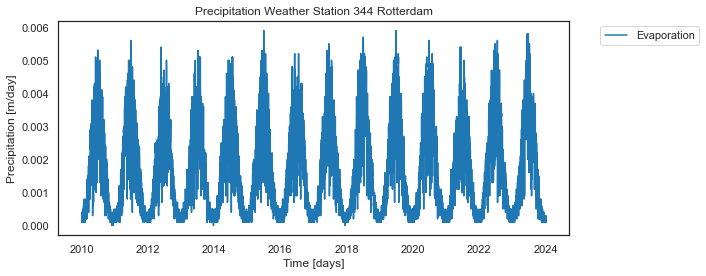
\includegraphics[width=\linewidth]{frontmatter/Heijplaat-fig/ET.png}
        \caption{Potential evaporation [m/day] over a period of 2010-2024, measured by KNMI weather station 344 in Rotterdam, The Netherlands.}
        \label{ET}
    \end{minipage}
\end{figure}


\subsubsection{Reverse forecasting}
A part of the Pastas package is reverse forecasting or also called backcasting of the observed data. Reversed forecasting takes place for all the unique monitoring wells present in the case study area. For every monitoring well, three figures are created: a) Reversed backcasting for data loggers; b) Reversed backcasting for manual measurements; c) A combination figure of the first figures combined, see figures \labelcref{dlheij}-\labelcref{combiheij}. Examples are shown for monitoring well 125563-96. 

\begin{figure}
    \centering
    % First figure
    \begin{minipage}{0.32\textwidth}
        \centering
        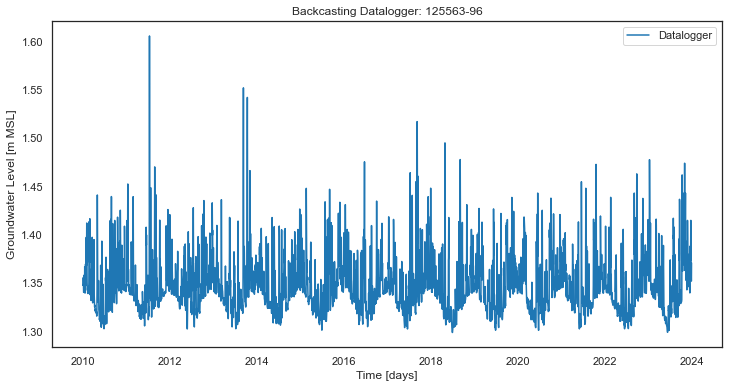
\includegraphics[width=\linewidth]{frontmatter/Heijplaat-fig/dl12556396.png}
        \caption{Reversed forecasting data based on data logger data for monitoring well 125563-96}
        \label{dlheij}
    \end{minipage}
    \hfill
    % Second figure
    \begin{minipage}{0.32\textwidth}
        \centering
        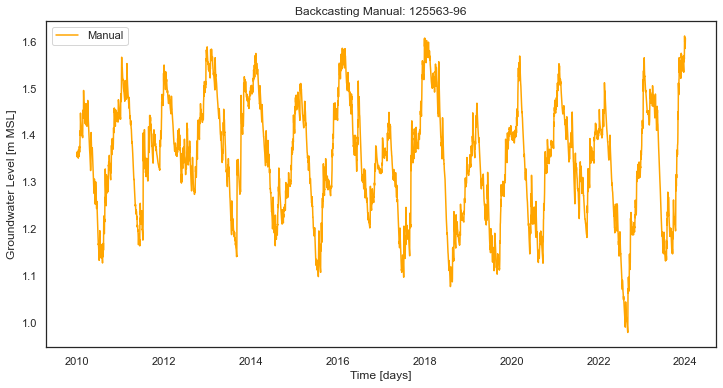
\includegraphics[width=\linewidth]{frontmatter/Heijplaat-fig/man12556396.png}
        \caption{Reversed forecasting data based on manual measurement data for monitoring well 125563-96}
        \label{hpheij}
    \end{minipage}
    \hfill
    % Third figure 
    \begin{minipage}{0.32\textwidth}
        \centering
        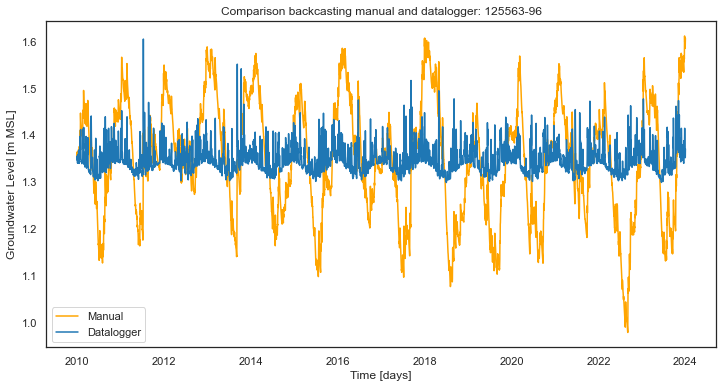
\includegraphics[width=\linewidth]{frontmatter/Heijplaat-fig/pastascombi96.png}
        \caption{Reversed forecasting data based on manual measurement data and datalogger data for monitoring well 125563-96.}
        \label{combiheij}
    \end{minipage}
\end{figure}

\clearpage
\subsubsection{Performance metrics}
The barplots shows the performance metrics RMSE, $R^2$, and EVP for all unique monitoring wells with a comparison to a distinction in dataloggers and manual collection method. The first bar plot shows the distribution of RMSE and $R^2$ for every unique monitoring well with a distinction between dataloggers and manual collection. The second bar plot shows the distribution of RMSE and $R^2$ for every unique monitoring well only. The third barplot \labelcref{barevpheij} describes the EVP for every monitoring well with a distinction between the manual collection method and datalogger. Generally, low values of the RMSE indicate a better fit of the model. The $R^2$ values represent the proportion of variance in the observed data that is predictable from the model inputs, with higher values indicating a better fit. Based on the bar plot, the performance of the models for each monitoring well can be compared. Overall, short bars for RMSE (blue and green) and tall bars for $R^2$ (red and orange) indicate a better model performance. An additional bar plot describes the EVP [\%] across the dataset. The EVP is a goodness-of-fit indicator which compares the variance of the observed data and the variance of the residual data (Asmuth von et al., 2012). A low EVP indicates that data could be missing in the data set, where the spatial pattern in the data set could be a possible reason. A statistical test is a follow-up, substantiating the difference between the performance of the two data groups.


\begin{figure}[htbp]
    \centering
    % First figure
    \begin{minipage}{0.48\textwidth}
        \centering
        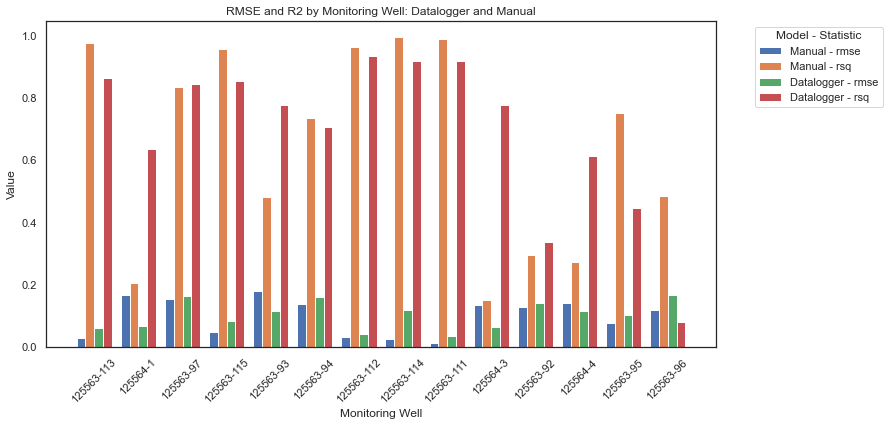
\includegraphics[width=\linewidth]{frontmatter/Heijplaat-fig/rmser2heij.png}
        \caption{Bar plot showing the metrics RMSE and $R^2$ for 14 monitoring wells.}
        \label{bar1heij}
    \end{minipage}\hfill
    % Second figure
    \begin{minipage}{0.48\textwidth}
        \centering
        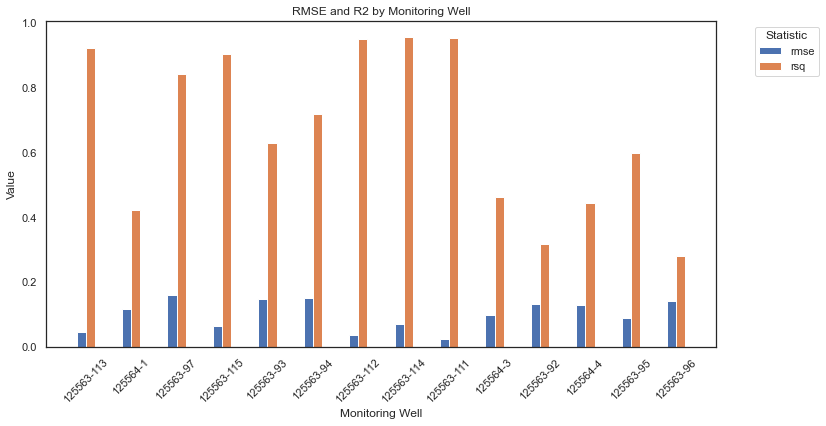
\includegraphics[width=\linewidth]{frontmatter/Heijplaat-fig/rmr2heij.png}
        \caption{Bar plot showing metrics RMSE and $R^2$ for 14 monitoring wells with a division in data logger and manual collection method.}
        \label{bar2heij}
    \end{minipage}\hfill
    % Third figure
    \begin{minipage}{0.48\textwidth}
        \centering
        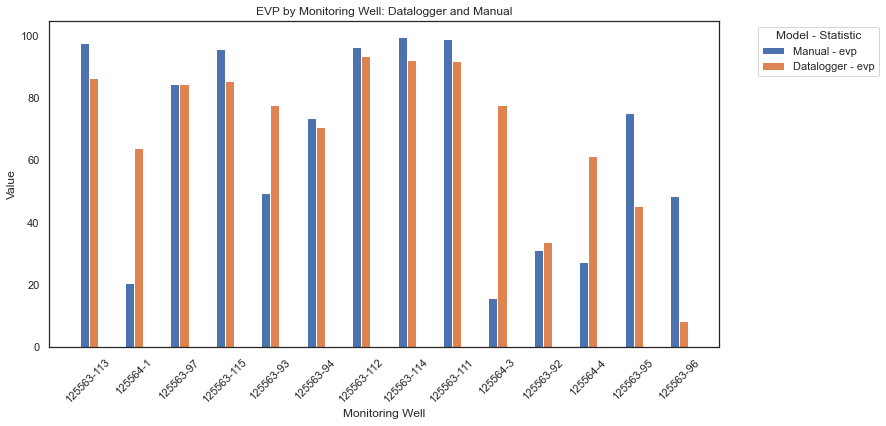
\includegraphics[width=\linewidth]{frontmatter/Heijplaat-fig/evpheij.png}
        \caption{Bar plot showing metric EVP for 14 monitoring wells.}   
        \label{barevpheij}
    \end{minipage}
\end{figure}

Figure \labelcref{welchheij} displays the result of the Welch's t-test, based on alpha = 0.05. The results of the performance metrics are labeled as RMSE, $R^2$, and EVP. Each performance metric provides the results of the t-statistic and p-value of the Welch's statistical test. The RMSE (blue section), explains that the t-statistic is low and a minimal difference is present between the dataloggers and manual collection method. The p-value is higher than alpha, indicating that the difference is not statistically significant. There is no evidence that one of the data groups provides more accurate measurements. The $R^2$ (orange section) explains that the t-statistic is positive, it is a small t-statistic and shows a difference between the two data groups. The p-value is slightly higher than alpha = 0.05, indicating no significant difference. The last metric is the EVP (green section). The t-statistic of the EVP has a positive value as well as a p-value higher than alpha. The percentage of the total variance in the observed data does not differ between the two data collection methods.

\clearpage

\begin{figure}[htbp]
    \centering
    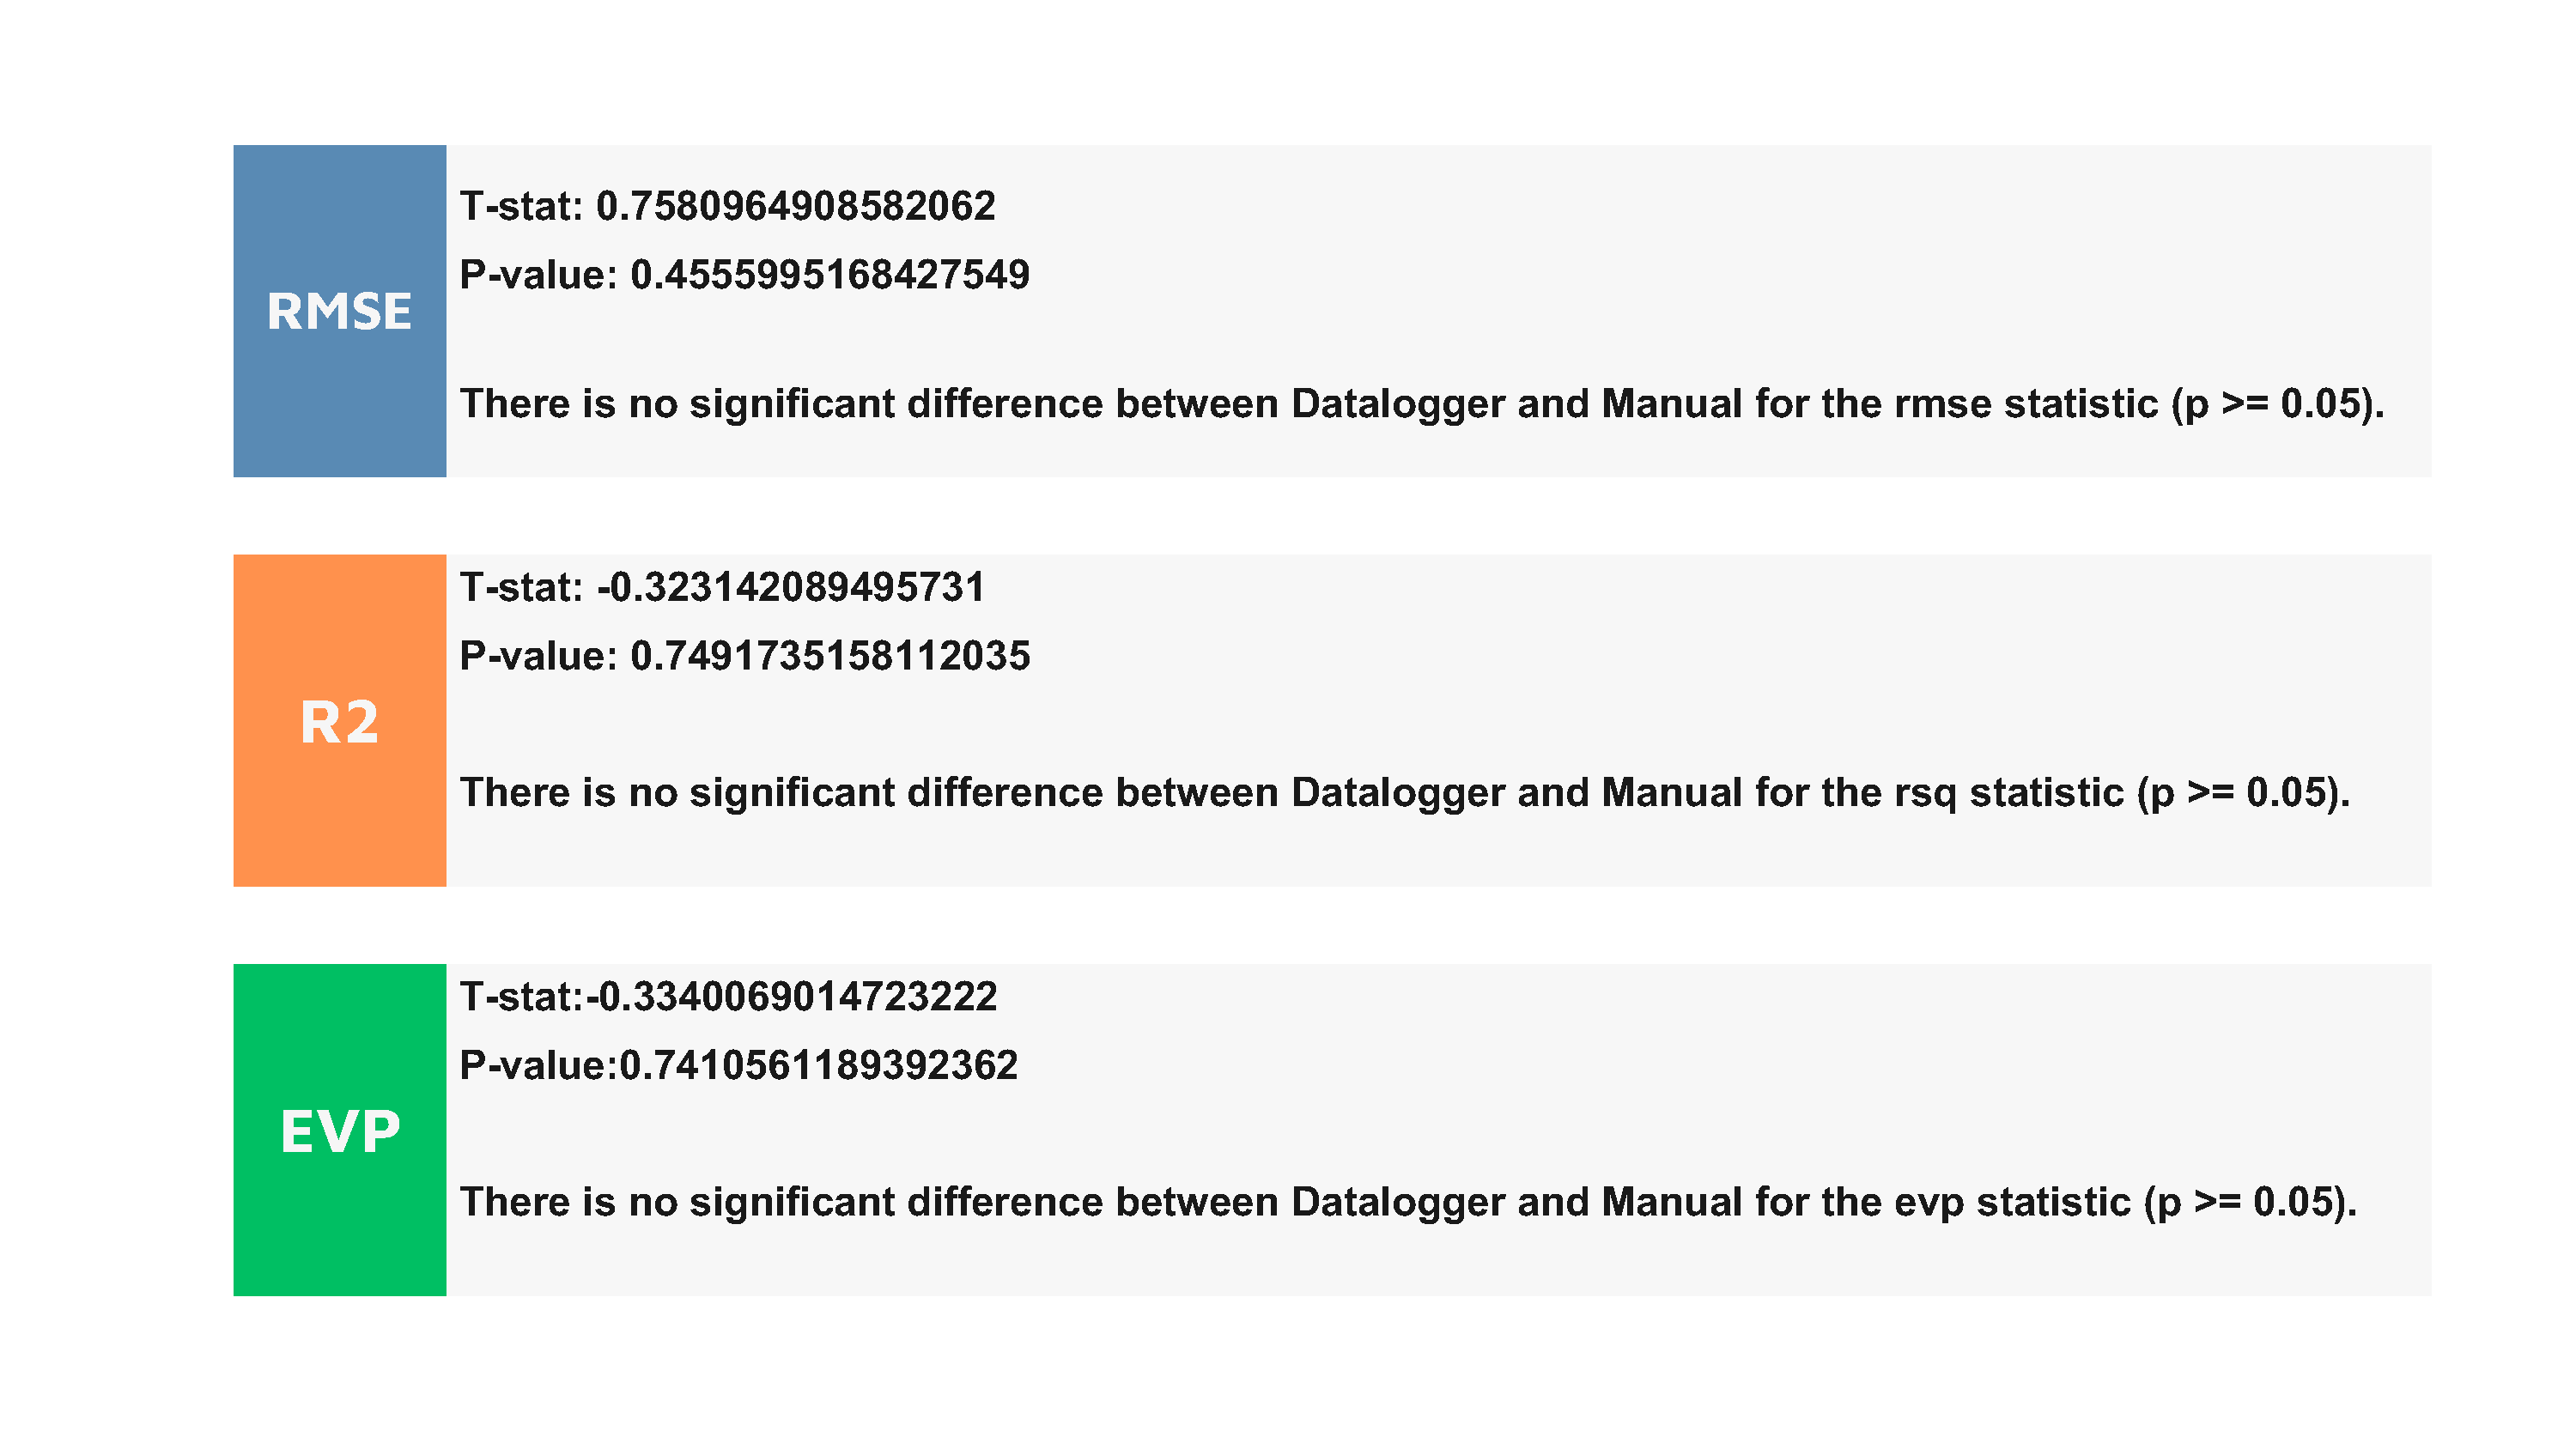
\includegraphics[width=0.80\linewidth]{frontmatter/Heijplaat-fig/heijstat.pdf}
    \caption{Overview of the performance of RMSE, $R^2$, EVP after the Welch's t-test and the difference between data loggers and manual collection method.} 
    \label{welchheij}
\end{figure}

According to the Welch's t-test, no substantial discrepancies were found in the data groups. None of the p-values are below the cut-off of alpha = 0.05. Consequently, just like the case study 'Rozenburg', it was decided to proceed with the group that is specialized in data loggers. Despite statistical significance, other factors are crucial in environmental sciences. Hence, the datalogger group is chosen, merging observed and simulated data into one dataset and excluding the manual measurements.

\subsubsection{Creation of new data frame}
The scatter plot below visualizes the observed data logger with the pink scatter and the simulated data of the data loggger is visualized by the green scatter. On the x-axis the time period [days] is shown and on the y-axis the groundwater level [m MSL]. Figure \labelcref{scatterheij} visualizes only monitoring well 125563-96, the remaining monitoring wells of the neighborhood are available through GitHub.


\begin{figure}[htbp]
    \centering
    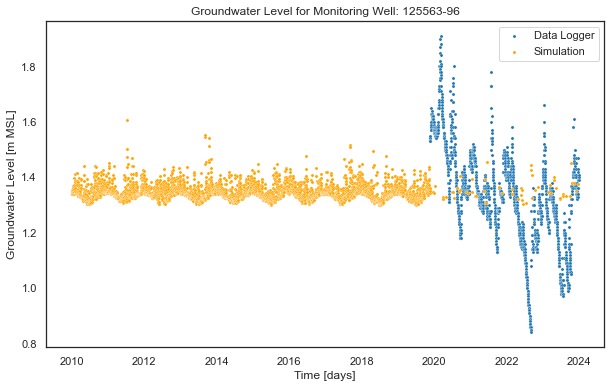
\includegraphics[width=0.80\linewidth]{frontmatter/Heijplaat-fig/scattercombi12556396.png}
    \caption{Scatter plot of simulated and observed data by data loggers for monitoring well 125563-96. The x-axis shows a period of 2010-2024 and the y-axis shows a range of 0.8 to 1.8 meters MSL.}  
    \label{scatterheij}
\end{figure}


\subsection{QR factorization}
Using QR factorization as foundation, a hierarchical list of the monitoring wells in Heijplaat is created. The optimal reduction percentage is determined and reduction tests can be executed. Resulting in an overview of eliminated monitoring wells and their capability to reconstruct future groundwater levels in the network.

\subsubsection{1D hydrograph data}
Figure \labelcref{gwlheij} is a geographical representation (epsg=28992) visualizing the spatial distribution of monitoring wells in the neighborhood "Heijplaat", plotted on a x,y coordinate system. Within the map, a scatter plot with a color scale represents the groundwater level measurements taken at the monitoring wells. The color scale has a range between -0.5 m to +3.0 m MSL. Each monitoring well represents a location as well as the color of monitoring well represents the value on the color scale. At the south side of the neighborhood, the GWL is increasing from approximately 2.0 meters to 3.0 meters [MSL]. For Heijplaat the increasing GWL is not necessarily defined through the digital terrain model in figure \labelcref{ahnheij}.
\begin{figure}[htbp]
    \centering
    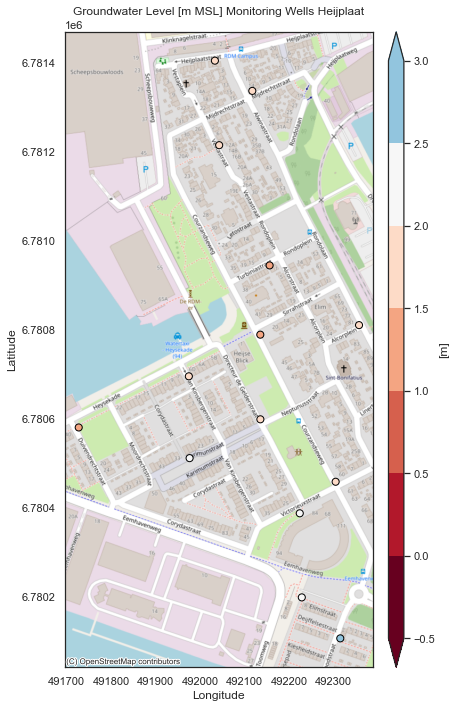
\includegraphics[width=0.50\linewidth]{frontmatter/Heijplaat-fig/gwlheij.png}
    \caption{Groundwater level [m MSL] across Heijplaat, using a color-coded system to represent the mean GWL observations for 14 monitoring wells.}
    \label{gwlheij}
\end{figure}


\clearpage

\subsubsection{Sampling data}
Preprocessing of the data includes transforming the data frame into an array, implementing both global and local centering methods, and splitting the dataset into an 80/20 ratio training and test set distribution. The result of the preprocessing is as follows, see tabel \labelcref{dataheij}.

\begin{table}[htbp]
\centering
\caption{Summary of sampling data.}
\label{dataheij}
\begin{tabular}{|l|l|}
\hline
\textbf{Parameter}                           & \textbf{Value}                                \\ \hline
Sampling period                              & 2020-01-02 00:00:00 to 2024-01-01 00:00:00   \\ \hline
Number of samples                            & 1462                                          \\ \hline
Number of features (sensors)                 & 14                                            \\ \hline
Shape of X (samples, sensors)                & (1462, 14)                                    \\ \hline
Min. and max. value                          & 0.7 [m]; 3.36 [m] \\ \hline
Min. and max. centered value                 & -0.768 [m] 0.589 [m]                         \\ \hline
Min. and max. centered value (exact)         & -0.7679038683451884 [m]; 0.5894112429907086 [m] \\ \hline
Mean centered data                           & 0.0 [m]                                     \\ \hline
Train data, Test data                        & 1169 , 293                                   \\ \hline
Train data, Test data (percentage)           & 80\%, 20\%                                  \\ \hline
\end{tabular}
\end{table} 

\subsubsection{Hierarchy of monitoring wells}
Figure \labelcref{rankheij} is a geographical representation (epsg=28992) of data points plotted on a x,y coordinate system. The horizontal axis is labeled as longitude and the vertical axis is labeled as latitude. The data points are scattered across the study area within a polygonal boundary that represents the neighborhood "Heijplaat". Each monitoring well monitoring well is color-coded according to the color bar on the right side of the plot. The color indicates the rank of each monitoring well. The color bar has a range between dark blue for the lowest values (0) to yellow for the highest values (14). The distribution of the color code does not follow a clear pattern within the study area. Some clusters of higher or lower ranked monitoring wells are present. Overall, the monitoring wells with additional value are marked blue. They show possibly show flashiness in their data, meaning a high frequency and rapidity in short term changes with strong irregular patterns. According to Ohmer et al. (2022), these monitoring wells indicate strong interaction with surface waters and boundary inflows. As well as a high seasonality and low variability. The monitoring wells that likely do not have additional value to the network are marked yellow. These wells show low flashiness and high seasonality. A cluster of redundant monitoring wells appears to be located at the southern side of the neighborhood. The data cluster could indicate a region of low data variability and flashiness. Towards the north of the neighborhood, a higher rank is also noted. 

\begin{figure}
    \centering
    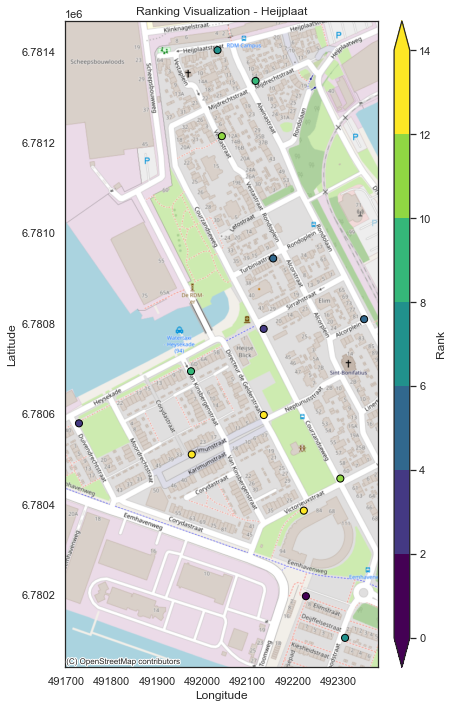
\includegraphics[width=0.75\linewidth]{frontmatter/Heijplaat-fig/rankheij.png}
    \caption{Visualization of the hierarchical list of 14 monitoring wells across Heijplaat.}    
    \label{rankheij}
\end{figure}

\clearpage

\subsubsection{Determining the optimal reduction rate}
Figures \labelcref{heij10}-\labelcref{heij90} visualize the Reconstruction Error of Heijplaat, plotting the root mean square error (RMSE) in meters on the y-axis against the number of monitoring wells on the x-axis. The line graph shows a decreasing function in the RMSE as the number of monitoring wells increasing, suggesting that more monitoring wells contribute to a lower reconstruction error in the data. In the figures, the orange marked point marks the optimal number of monitoring wells where the reconstruction error reaches the threshold that is indicated by the orange line. The threshold is an acceptable level of RMSE for the reconstruction process. The original groundwater monitoring network of Heijplaat includes 14 monitoring wells. 
\newline
Starting with a reduction rate of 10\%, the network is reduced to 12 monitoring wells with a reconstruction error of below 0.02 meters, see figure \labelcref{heij10}. Figure \labelcref{heij25} describes a reduction of 25\% explains that a number of 10 monitoring wells is the most optimal with a removal of 4 monitoring wells. The RMSE is calculated to determine the optimal number of monitoring wells in the neighborhood. Figure \labelcref{heij50}, demonstrates a function based on a reduction rate of 50\%. The RMSE decreases as more monitoring wells are added to the network. At the point of n = 7 on the x-axis, an orange dot is indicated. Beyond this point, the decrease in RMSE slows down, suggesting returns on error reduction after a specific number of monitoring wells is reached. 


\begin{figure}[htbp]
    \centering
    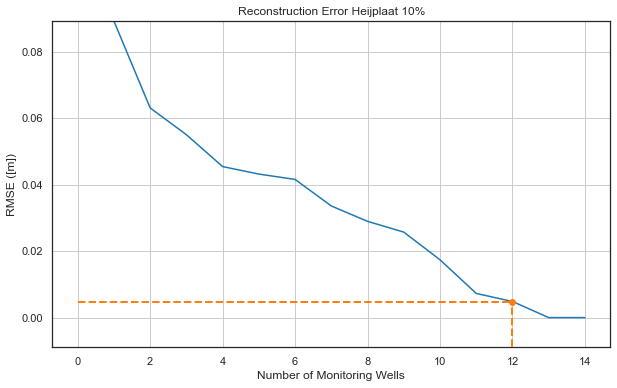
\includegraphics[width=0.5\linewidth]{frontmatter/Heijplaat-fig/heij10.png}
    \caption{RMSE based on a network reduction of 10\%. The optimal number of wells is 12.}
    \label{heij10}
\end{figure}

\begin{figure}[htbp]
    \centering
    \begin{minipage}{0.45\linewidth}
        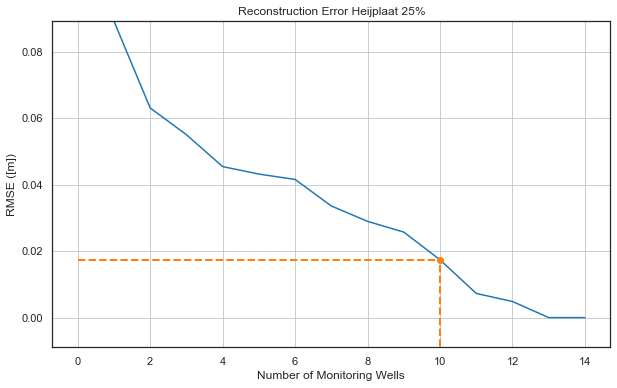
\includegraphics[width=\linewidth]{frontmatter/Heijplaat-fig/25heij.png}
        \caption{RMSE based on a network reduction of 25\%. The optimal number of wells is 10.}
        \label{heij25}
    \end{minipage}
    \hfill
    \begin{minipage}{0.45\linewidth}
        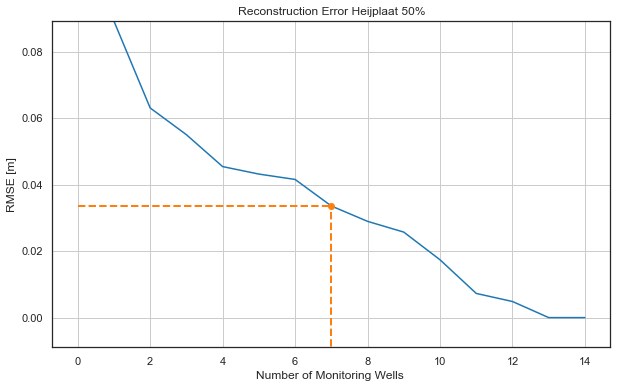
\includegraphics[width=\linewidth]{frontmatter/Heijplaat-fig/50heij.png}
        \caption{RMSE based on a network reduction of 50\%. The optimal number of wells is 7.}
        \label{heij50}
    \end{minipage}
\end{figure}

Figure \labelcref{heij75}, displays a similar function where the RMSE decreases as the number of monitoring wells increases. The RMSE declines as the monitoring well count approach reaches the point above 3 monitoring wells. This is the point marked with the orange dashed line. The line marks the optimal number of monitoring wells where the reconstruction error reaches the threshold value. The threshold value is an acceptable level of RMSE for the reconstruction process. Initially, Heijplaat includes 14 monitoring wells. The results of the RMSE explains that only 3 monitoring wells remain, 11 monitoring wells have to be removed from the local network if a reduction of 75\% is being used in the approach. A reduction rate of 75 \% explains an equilibrium state between the number of monitoring wells and the reconstruction error is achieved. 
\newline
Continuing with figure \labelcref{heij90}, the reconstruction error for a reduction of 90\% is displayed. The figure plots the RMSE in meters on the y-axis against the number of monitoring wells on the x-axis. The line graph shows a decreasing function in the RMSE as the number of monitoring wells increases. The orange marked point marks the optimal number of monitoring wells where the reconstruction error reaches the threshold that is indicated by the orange line. The threshold is the acceptable level of RMSE for the reconstruction process. Heijplaat includes 14 monitoring wells. The results of the reduction rate describes that 1 monitoring well remains, while 13 monitoring wells are eliminated from the network.

\begin{figure}[htbp]
    \centering
    \begin{minipage}{0.45\linewidth}
        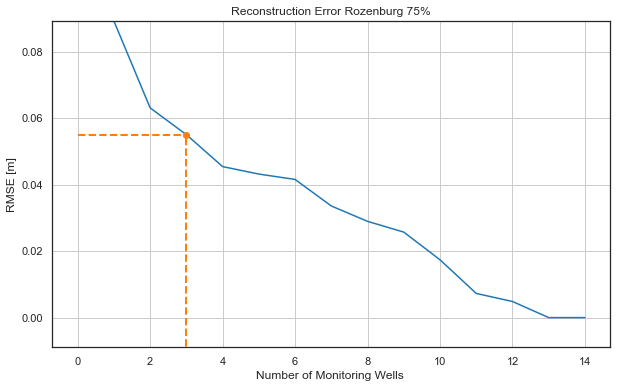
\includegraphics[width=\linewidth]{frontmatter/Heijplaat-fig/75heij.png}
        \caption{RMSE based on a network reduction of 75\%. The optimal number of wells is 3.}
        \label{heij75}
    \end{minipage}
    \hfill
    \begin{minipage}{0.45\linewidth}
        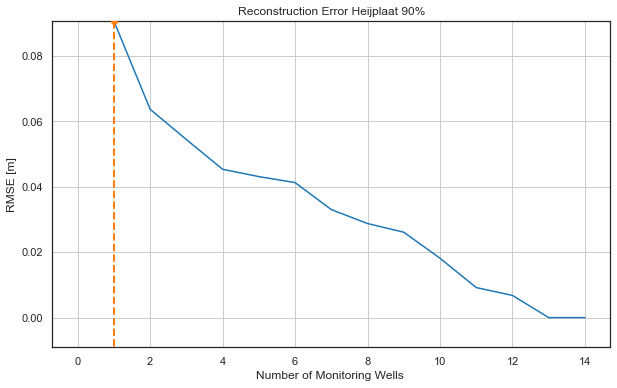
\includegraphics[width=\linewidth]{frontmatter/Heijplaat-fig/heij90.png}
        \caption{RMSE based on a network reduction of 90\%. The optimal number of wells is 1.}
        \label{heij90}
    \end{minipage}
\end{figure}


\subsubsection{The optimal reduction rate}
The optimal reduction rate for a monitoring network consisting of 14 monitoring wells counts up to a value where both RMSE and MAE reach a point of stabilization. Figure \labelcref{rmseheij} visualizes all reduction rates between a range of 10-90\% with their corresponding reconstruction error and mean absolute error. The upper values of each reduction rate correlate to the MAE, while the lower values - marked by the dashed line- describe the reconstruction error.  A reduction rate of 25\% implies that the optimal number of monitoring wells is 10, meaning that 4 monitoring wells might be eliminated, see figure 5.48. Additionally, the RMSE counts up to X and the MAE to X meters. As stated in the chapter \textit{Research Methodology}, the reconstruction capability of the eliminated monitoring wells is tested through the creation of hydrographs. In figures \labelcref{hwell1}-\labelcref{hwell4}, hydrographs are shown. The hydrographs include a measured (blue line) and reconstructed (red line) function. The reconstructed functions are based on observed data and the goodness-of-fit of the model. Performance metrics regarding the MAE, RMSE, R2 and rBIAS determine the goodness-of-fit of the functions, they are available underneath the figures \labelcref{hwell1}-\labelcref{hwell4}. 

\begin{figure}[h]
    \centering
    \includegraphics[width=0.60\linewidth]{frontmatter/Heijplaat-fig/rrheij.png}
    \caption{Overview of RMSE and MAE for a range of reduction rates (10-25-75-90\%).}
    \label{rmseheij}
\end{figure}
\newpage
A reduction rate of 25\% implies that the optimal number of monitoring wells is 10, meaning that 4 monitoring wells might be eliminated, see figure \labelcref{heij25}. Additionally, the RMSE counts up to X and the MAE to X meters. As stated in the chapter \textit{Research Methodology}\textit{}, the reconstruction capability of the eliminated monitoring wells is tested through the creation of hydrographs. In figures \labelcref{hwell1}-\labelcref{hwell4} hydrographs are shown. The hydrographs include a measured (blue line) and reconstructed (red line) function. The reconstructed functions are based on observed data and the goodness-of-fit of the model. Performance metrics regarding the MAE, RMSE, R2 and rBIAS determine the goodness-of-fit of the functions, they are available underneath the figures \labelcref{hwell1}-\labelcref{hwell4}. \\
\\
As can be seen from the figures, the plots have comparable functions; a decreasing groundwater level from April to July 2023. An increase occurs in July towards mid August 2023. During the start of Fall, a small increase in groundwater level occurs in October with strong increases in November and December 2023. In January 2024, the groundwater level is just as high as at the beginning of November 2023. Based on the performance metrics of the potentially eliminated monitoring wells, it can be seen that the MAE and RMSE are constant values throughout the network. The MAE reaches a value of X meters and the RMSE counts up to X meters. The coefficient of determination differs for every monitoring well, but ranges between X and X meters. An average R2 of X meters is calculated.
\begin{figure}[h]
    \centering
    % Eerste rij
    \begin{minipage}{0.48\linewidth}
        \includegraphics[width=\linewidth]{frontmatter/Heijplaat-fig/125563111.png}
        \caption{Eliminated monitoring well: 125563-111.}
        \label{hwell1}
    \end{minipage}
    \hfill
    \begin{minipage}{0.48\linewidth}
        \includegraphics[width=\linewidth]{frontmatter/Heijplaat-fig/125563112.png}
        \caption{Eliminated monitoring well: 125563-112.}
        \label{125563-112}
    \end{minipage}
    
    % Tweede rij
    \begin{minipage}{0.48\linewidth}
        \includegraphics[width=\linewidth]{frontmatter/Heijplaat-fig/125563113.png}
        \caption{Eliminated monitoring well: 125563-113.}
        \label{125563-113}
    \end{minipage}
    \hfill
    \begin{minipage}{0.48\linewidth}
        \includegraphics[width=\linewidth]{frontmatter/Heijplaat-fig/125564-3.png}
        \caption{Eliminated monitoring well: 125564-3.}
        \label{hwell4}
    \end{minipage}
\end{figure}
\newpage
The measured and reconstructed groundwater levels are tested with the Welch's t-test to determine whether it is the case of a significant difference between the measured and reconstructed groundwater levels. The results are displayed in table \labelcref{theij}.  X out of X eliminated monitoring wells experience a significant difference between the measured and reconstructed groundwater level data. This means that the p-values of the monitoring wells are lower than alpha = 0.05.
\begin{table}
    \centering
        \caption{Overview of statistical results of the eliminated monitoring wells with a network reduction of 25\%. The overview explains the p-value of the monitoring wells if they experience a significant difference between the observed and reconstructed data. }
    \begin{tabular}{|c|c|} \hline 
         Monitoring Well& Result t-Test\\ \hline 
         125563-111& Significant difference (p-value = 0.000)\\ \hline 
         125563-112& Significant difference (p-value = 0.000)\\ \hline 
         125563-113& Significant difference (p-value = 0.000)\\ \hline 
         125564-3& Significant difference (p-value = 0.000)\\ \hline
    \end{tabular}
    \label{theij}
\end{table}
Continuing with a box plot of the coefficient of determination, the $R^2$. Box plot \labelcref{boxheij} visualizes the distribution of the $R^2$ across the dataset after a reduction of 25\% took place. On the y-axis, the score in meters is shown, which ranges between X and X meters. The orange line explains a median value of around 0.974 meters. The whiskers at the bottom and top of the box do not have equal lengths. The bottom whisker ranges from X to X meters, while the whisker at the top ranges from X to X meters approximately. 

\begin{figure}[htbp]
    \centering
    \includegraphics[width=0.70\linewidth]{frontmatter/Heijplaat-fig/R2.png}
    \caption{Performance metric $R^2$. The orange line indicates the median value. The y-axis ranges from X to X meters.}
    \label{boxheij}
\end{figure}

\clearpage
\subsubsection{Mean Absolute Error of Reduction}
Based on the reduction percentage of 25\%, reconstruction hydrographs could be plotted in figures \labelcref{hwell1}-\labelcref{hwell4}. The extent to which the reconstructed groundwater level data corresponds to the actual observed data can be determined by the mean absolute error [meters]. The mean absolute error is calculated for every, eliminated monitoring well. A color rank visualizes the level of the calculated mean absolute error (epsg=28992) in figure \labelcref{maeheij}. Blue indicates a low MAE, while yellow indicates a high MAE. The visualization enables the identification of monitoring wells with higher or lower predictive accuracy, which could influence decision-making regarding the placement of future monitoring wells or the scope of maintenance efforts on existing wells. The MAE measures indirectly the performance of monitoring wells regarding data reconstruction. A high MAE in a network of lower MAE values can suggest a vulnerable monitoring well for external, environmental factors. Monitoring wells with a high MAE address the reliability of data. The monitoring well that is marked with a yellow color indicates a higher MAE value compared to the other monitoring wells. 

\begin{figure}[htbp]
    \centering
    \includegraphics[width=0.5\linewidth]{frontmatter/Heijplaat-fig/mae25heij.png}
    \caption{Mean Absolute Error [meters] across Heijplaat, using a color-coded system to represent the calculated MAE for the eliminated monitoring wells.}
    \label{maeheij}
\end{figure}
\clearpage

\subsubsection{Optimized Network}
After the network is reduced, 75\% of the monitoring wells will remain in the GWMN after reduction takes place. A geographical representation (epsg=28992) of the monitoring wells is available in figure \labelcref{afterheij}. The blue sites indicate the location of the remaining monitoring wells in the network. Originally, the neighborhood Heijplaat had a density of one monitoring well/11.21 $m^2$. After the reduction-optimization process, the network changes to one monitoring well/15.7 $m^2$.


\begin{figure}[htbp]
    \centering
    \includegraphics[width=0.60\linewidth]{frontmatter/Heijplaat-fig/After.png}
    \caption{Map depiction of the remaining monitoring wells in Heijplaat after following a 25\% reduction of the network.}
    \label{afterheij}
\end{figure}



